% This work is licensed under the Creative Commons
% Attribution-NonCommercial-ShareAlike 4.0 International License. To view a copy
% of this license, visit http://creativecommons.org/licenses/by-nc-sa/4.0/ or
% send a letter to Creative Commons, PO Box 1866, Mountain View, CA 94042, USA.

% (c) Eric Kunze, 2019

%%%%%%%%%%%%%%%%%%%%%%%%%%%%%%%%%%%%%%%%%%%%%%%%%%%%%%%%%%%%%%%%%%%%%%%%%%%%%%%
% Template for lecture notes and exercises at TU Dresden.
%%%%%%%%%%%%%%%%%%%%%%%%%%%%%%%%%%%%%%%%%%%%%%%%%%%%%%%%%%%%%%%%%%%%%%%%%%%%%%%

\documentclass[ %
ngerman, %
a4paper, %
sectionreset, %
chapterstyle=framed, %
sectionstyle=pure, %
titlefont=osfamily %
]{../../texmf/tex/latex/mathscriptMathTUD/mathscriptMathTUD}

\usepackage[order=firstname, fractionappearence=lowerraise]{../../texmf/tex/latex/mathworkMathTUD/mathworkMathTUD}
%\usepackage[presentExercise]{../../texmf/tex/latex/exercisesMathTUD/exercisesMathTUD}

%%%%%%%%%%%%%%%%%%%%%%%%%%%%%%%%%%%%%%%%%%%%%%%%%%%%%%%%%%%%%%%%%%%%%%%%%%%%%%%

%---------------------------------------
% additional packages
%---------------------------------------

% none


%---------------------------------------
% general settings
%---------------------------------------

\name{Eric Kunze}
\matnr{Nummer}
\email{\href{mailto:eric.kunze@mailbox.tu-dresden.de}{\ttfamily eric.kunze@mailbox.tu-dresden.de}}

\modul{Proseminar: Numerik}
\period{Sommersemester 2019}

%\tutor{Dr. Legrand}
%\group{Tag x. DS, (un)gerade Woche}

\lecturer{Prof. Dr. Andreas Fischer}
\faculty{Mathematik}
\institute{Numerik}
\professorship{Numerik der linearen Optimierung}

%%%%%%%%%%%%%%%%%%%%%%%%%%%%%%%%%%%%%%%%%%%%%%%%%%%%%%%%%%%%%%%%%%%%%%%%%%%%%%%
% specific commands

\counterwithin{themcount}{chapter}
\titleformat{\chapter}[frame]{\bfseries\titlefont\color{cddarkblue}}{\enskip \LARGE Vortrag \;\thechapter \enskip}{8pt}{\Huge\centering\MakeUppercase}%
\titlespacing{\chapter}{0pt}{0pt}{10pt}%
\usepackage{afterpage}

\newcommand\blankpage{%
	\null
	\thispagestyle{empty}%
	\addtocounter{page}{-1}%
	\newpage}

\newcommand{\zerodisplayskips}{%
	\setlength{\abovedisplayskip}{3pt}%
	\setlength{\belowdisplayskip}{3pt}%
	\setlength{\abovedisplayshortskip}{0pt}%
	\setlength{\belowdisplayshortskip}{0pt}}
\appto{\normalsize}{\zerodisplayskips}
\appto{\small}{\zerodisplayskips}
\appto{\footnotesize}{\zerodisplayskips}

\newcommand{\vortragender}[1]{\begin{center} \textit{\Large #1} \end{center}}

%%%%%%%%%%%%%%%%%%%%%%%%%%%%%%%%%%%%%%%%%%%%%%%%%%%%%%%%%%%%%%%%%%%%%%%%%%%%%%%


\begin{document}
    
    \MakeTitle[dark][Numerische Verfahren zur Lösung unrestringierter Optimierungsaufgaben]
    
    \tableofcontents
    
    \chapter{Optimalitätskriterien}

\vortragender{Johann Seidl}

In der heutigen Welt sind viele mathematische Probleme auf Real-World-Probleme zurückzuführen. Unser unter (\ref{formel1}) verstandenes \textit{Minimierungsproblem} spielt unter anderem Rollen in den Ingenieurwissenschaften, der Physik, der Medizin oder der Ökonomie. 

\section{Minimierungsproblem}
Unter einem Minimierungsproblem wird folgende Aufgabe verstanden.  

\begin{definition}
	Sei $ X \subseteq \Rn $ und eine Funktion $ f: X \to \R $, dann wird ein $x^\ast \in X $ mit folgender Eigenschaft gesucht
	\begin{equation} 
		f(x^\ast) \leq f(x)   \qquad \forall x \in X 
		\label{formel1}
	\end{equation}
\end{definition}

\begin{bemerkung}
	In kurzer Notation lautet diese Aufgabe $ \min f(x)$ unter der Nebenbedingung $x \in X$. Ist $X = \R$, dann spricht man von unrestringierten Problemen, andernfalls von restringierten Problemen. 
\end{bemerkung}

\section{Optimalitätskriterien}

In diesem Kapitel gehen wir auf notwendige und hinreichende Bedingungen für lokale Minima ein, welche Ableitungen benutzen. Der erste Satz bezieht ein notwendiges Kriterium erster Ordnung, wobei man von einem Kriterium erster Ordnung spricht, da nur Informationen über die erste Ableitung eingehen.

\begin{satz} \label{satz 1.3_2.1}
	Seien $ X \subseteq \R^n $ eine offene Menge und $ f:X \to \R $ eine stetig differenzierbare Funktion. Ist  $ x^\ast \in X $ ein lokales Minimum von $f$ (auf $X$), so gilt 
	\begin{equation*}
		\nabla f(x^\ast) = 0 
	\end{equation*}
	d.h., $x^\ast$ ist ein stationärer Punkt von $f$. 
\end{satz}
\begin{proof}
	Sei $ x^\ast \in X $ ein lokales Minimum von $f$, jedoch $\nabla f(x^\ast) \ne 0 $. Dann existiert ein Vektor $d \in \R^{n} $ mit 
	\begin{equation*}
		\nabla \trans{f(x^\ast)} d < 0
	\end{equation*}
	Eine mögliche Wahl für $d$ kann zum Beispiel $d \defeq -\nabla f(x^\ast)$ sein. Da $f$ nach Voraussetzung stetig differenzierbar ist, gilt für die Richtungsableitung $f'(x^\ast;d)$ von $f$ in $ x^\ast$ in Richtung $d$: 
	\begin{equation*}
		f'(x^\ast;d) = \lim_{t \to 0+}\ \dfrac{f(x^\ast + td) - f(x^\ast)}{t} = \nabla \trans{f(x^\ast)} d < 0. 
	\end{equation*}
	Folglich gibt es ein $\quer{t} >0 $ mit $ x^\ast +td \in X$ und 
	\begin{equation*}
		\dfrac{f(x^\ast+td) - f(x^\ast)}{t}<0 \qquad \forall t \in (0,\overline{t} ] 
	\end{equation*}
	Somit ist 
	\begin{equation*}
		f(x^\ast+td)<f(x^\ast) \qquad \forall t \in (0,\overline{t} ]
	\end{equation*}
	Dies steht aber im Widerspruch zur Voraussetzung, dass $x^\ast$ ein lokales Minimum von $f$ ist.
\end{proof}

\begin{bemerkung}
	Offensichtlich ist dieser Satz keine hinreichende Bedingung, da auch ein mögliches Maxima die oben genannten Voraussetzungen erfüllt.
\end{bemerkung}

\begin{erinnerung}
	Eine Matrix ist positiv semidefinit, falls für die symmetrische $ n \times n$ Matrix $M$ gilt 
	\begin{equation}
		\trans{x}Mx \ge 0 \qquad \forall x \in \R^{n} \setminus \menge{0}
		\label{definit}
	\end{equation}
\end{erinnerung}

\begin{erinnerung}[Satz von Taylor]
	Seien $f : \R^{n} \to \R$ zweimal stetig differenzierbar sowie $x,y \in \R^{n}$ gegeben. Dann existiert ein $\theta \in (0,1)$ mit 
	\begin{equation}
		f(x) = f(y) + \nabla \trans{f(y)}(x-y)+\dfrac{1}{2}\trans{(x-y)} \nabla^{2} f(\xi)(x-y)
		\label{Taylor}
	\end{equation}
	für $\xi = y+\theta(x-y)$.
\end{erinnerung}

Betrachten wir nun einen Satz, welcher eine notwendige Bedingung zweiter Ordnung nutzt. Man spricht wieder von Bedingung zweiter Ordnung, da der Satz Informationen über die zweiter Ableitung enthält.

\begin{satz} \label{satz 1.7_2.5}
	Seien $ X \subseteq \R^n $ eine offene Menge und $ f: X \to \R $ eine zweimal stetig differenzierbare Funktion. Ist  $ x^\ast \in X $ ein lokales Minimum von $f$ (auf $X$), so ist die Hesse-Matrix $\nabla^{2} f(x^\ast)$ positiv semidefinit.
\end{satz}
\begin{proof}
	Sei $x^\ast \in X$ ein lokales Minimum von $f$, jedoch $\nabla^{2}f(x^\ast)$ nicht positiv semidefinit (\ref{definit}). Dann existiert ein Vektor $d \in \R^{n}$ mit 
	\begin{equation}
		\trans{d} \nabla^{2} f(x^\ast) d < 0
		\label{formel2}
	\end{equation}
	Nutzt man nun (\ref{Taylor}) ergibt sich mit Satz 2.1 für alle hinreichend kleinen $t>0$:
	\begin{equation*}
	\begin{split}
		f(x^\ast+td)  &= f(x^\ast) + \nabla \trans{f(x^\ast)}(td) + \dfrac{1}{2}\trans{(td)} \nabla^{2} f(\xi_{t})(td) \\
		&= f(x^\ast) + \dfrac{1}{2}t^{2}\trans{d} \nabla^{2} f(\xi_{t})d 
		\end{split}
	\end{equation*}
	Dabei ist $\nabla \trans{f(x^\ast)}(td) = 0$, da $x^\ast$ schon das lokale Minimum ist. Des Weiteren ist $\xi_{t} = x^\ast + \upsilon_{t}td$ für ein $\upsilon_{t}$ mit $0 < \upsilon_{t} < 1$. Aus Stetigkeitsgründen folgt hieraus unter Verwendung von (\ref{formel2}) die Existenz eines $\overline{t} > 0$ mit 
	\begin{equation*}
		f(x^\ast+td)<f(x^\ast) \qquad \forall t \in (0,\overline{t}]
	\end{equation*}
	Dies steht aber im Widerspruch dazu, dass $x^\ast$ ein lokales Minimum ist.
\end{proof}

Auch die Bedingungen aus den Sätzen \ref{satz 1.3_2.1} und \ref{satz 1.7_2.5} zusammen sind \textit{nicht} hinreichend dafür, dass $x^\ast$ ein lokales Minimum ist.

\begin{beispiel}
	Betrachte $ f: \R^{2} \to \R $ mit $f(x) = x_{1}^{2} - x_{2}^{4}$, $x^\ast =(0,0)$. Die Ableitung erster Ordnung und die Hesse-Matrix der Funktion sind gegeben durch: 
	\begin{align*}
		f'(x) &= (2x_{1} , -4x_{2}^{3}) \\
		f''(x) &= \begin{pmatrix} 2 & 0 \\ 0 & -12 x_{2} \end{pmatrix}
	\end{align*}
	Man kann leicht erkennen, dass $f'(x^\ast)=0$ und die Eigenwerte der Matrix im Punkt $x^\ast$ $ \lambda_{1} =0$ und $\lambda_{1} =2$ sind, also die Matrix positiv semidefinit ist. Die Voraussetzungen für Satz \ref{satz 1.7_2.5} sind also erfüllt. Dennoch ist zum Beispiel für $X = \R^{2}$ $f(0,1) < f(0,0)$. 
\end{beispiel}

\begin{satz} \label{satz 1.9_2.7}
	Seien $ X \subseteq \R^n $ offen und $ f:X \to \R $ zweimal stetig differenzierbar. Gelten
	\begin{enumerate}[label=(\alph*), nolistsep, topsep=-\parskip]
		\item $\nabla f(x^\ast) =0$ und 
		\item $\nabla^{2} f(x^\ast)$ ist positiv definit, 
	\end{enumerate}
	so ist $x^\ast$ ein striktes lokales Minimum von $f$ (auf $X)$
\end{satz}

\begin{proof}
	Aus (b) folgt zunächst die Existenz einer Konstanten $\epsilon$ mit 
	\begin{equation*}
		\trans{d}\nabla^{2} f(x^\ast)d \ge \epsilon \trans{d}d \qquad \forall d \in \R^{n}
	\end{equation*}
	Nach (\ref{Taylor}) gilt für alle hinreichend nahe bei Null gelegenen $d \in \R^{n}$ :
	\begin{equation}
		f(x^\ast+d) = f(x^\ast) + \nabla \trans{f(x^\ast)}(d) + \dfrac{1}{2}\trans{d} \nabla^{2} f(\xi_{d})d
		\label{cauchy}
	\end{equation}
	mit $\xi_{t} = x^\ast + \upsilon_{d}td \,$ für ein $\upsilon_{d}$ mit $0 < \upsilon_{d} < 1$. Durch Voraussetzung (a) erhalten wir $\nabla \trans{f(x^\ast)}(td) = 0$. Wenden wir nun die Cauchy - Schwarz - Ungleichung auf (\ref{cauchy}) an, erhalten wir 
	\begin{equation*}
	\begin{split}
		f(x^\ast+d)  &= f(x^\ast) + \dfrac{1}{2}\trans{d} \nabla^{2} f(x^\ast)d+ \dfrac{1}{2} \trans{d} \big( \nabla^{2} f(\xi_{d}) - \nabla^{2} f(x^\ast) \big) d \\
		& \ge
		f(x^\ast) + \dfrac{1}{2}(\epsilon - \Vert \nabla^{2}f(\xi_{d}) - \nabla^{2}f(x^\ast) \Vert) \Vert d \Vert ^{2}
	\end{split}
	\end{equation*}
	Folglich gilt 
	\begin{equation*}
		f(x^\ast +d) > f(x^\ast) \qquad \forall d\neq 0 \text{ und  hinreichend nahe }  0
	\end{equation*}
	Also ist $x^\ast$ ein striktes lokales Minimum von $f$.
\end{proof}

\begin{bemerkung}
	Dieser Satz liefert ein hinreichendes Kriterium. Man beachte jedoch, dass die Bedigungen (a) und (b) aus Satz \ref{satz 1.9_2.7} nicht notwendig für die strikte lokale Minimaliltät von $x^\ast$ sind. Genauere Erklärungen liefert nachfolgendes Beispiel.
\end{bemerkung}

\begin{beispiel}
	Betrachte $ f: \R^{2} \to \R $ mit $f(x) = x_{1}^{2} + x_{2}^{4}$, $x^\ast =(0,0)$.  Dann ist
	\begin{align*}
		f'(x) &=(2x_{1} , 4x_{2}^{3}) \\
		f''(x) &= \begin{pmatrix} 2 & 0 \\ 0 & 12x_{2} \end{pmatrix}
	\end{align*}
	so stellt man fest, dass $\nabla^{2} f(x^\ast)$  positiv semidefinit ist und somit Satz \ref{satz 1.9_2.7} keine Anwendung finden kann (Voraussetzung (b) verletzt). Man erkennt jedoch leicht, dass $(0,0)$ das globale Minimum ist.
\end{beispiel}
    \chapter{Konvexe Funktionen}

\vortragender{Eric Kunze}

In diesem Vortrag beschäftigen wir uns mit der Klasse der konvexen Funktionen, deren Rolle in der Optimierung in späteren Vorträgen behandelt werden wird. \\
% Es sei vorweggenommen, dass insbesondere die notwendige Optimalitätsbedingung für konvexe Funktionen schon hinreichend ist.
%
Zunächst benötigen wir eine gewisse Struktur auf den Definitionsbereichen von konvexen Funktionen. Diese wird durch \textit{konvexe Mengen} realisiert.

\begin{definition}[konvexe Menge]
	Eine Menge $X \subseteq \Rn$ heißt \begriff{konvex}, wenn für alle $x,y \in X$ und alle $\lambda \in (0,1)$ auch
	\begin{align} \label{eq: def_konvexkombination}
		\lambda x + (1 - \lambda) y \in X
	\end{align}
	Eine solche Linearkombination $\sum_{i=1}^{n} \mu_i x_i$ von Vektoren $x_i \in \Rn$ mit $\mu_i \in (0,1)$ für alle $i \in \menge{1,\dots,n}$ und $\sum_{i=1}^n \mu_i = 1$ nennt man auch \begriff{Konvexkombination}
\end{definition}

Anschaulich kann die Definition wie folgt gedeutet werden:
Eine Menge ist genau dann konvex, wenn jede Verbindungsstrecke zweier Punkte der Menge wieder vollständig in der Menge liegt.

% TODO Abbildung

Ausgehend davon können wir nun eine neue Klasse von Funktionen definieren.

\begin{definition}[konvexe Funktion] \label{def: konvexe_fkt}
	Sei $X \subseteq \Rn$ eine konvexe Menge. Eine Funktion $\abb{f}{X}{\R}$ heißt
	\begin{itemize}[leftmargin=*, nolistsep]
		\item \begriff{konvex} (auf $X$), wenn für alle $x,y \in X$ und alle $\lambda \in (0,1)$ gilt, dass
		\begin{align} \label{eq: konvexe_fkt}
			f(\lambda x + (1-\lambda)y) \leq \lambda f(x) + (1-\lambda) f(y)
		\end{align}
		\item \begriff{strikt konvex} (auf $X$), wenn für alle $x,y \in X$ mit $x \neq y$ und alle $\lambda \in (0,1)$ gilt, dass
		\begin{align} \label{eq: strikt_konvex}
			f(\lambda x + (1-\lambda)y) < \lambda f(x) + (1-\lambda) f(y)
		\end{align}
		\item \begriff{gleichmäßig konvex} (auf $X$), wenn es ein $\mu > 0$ gibt mit 
		\begin{align} \label{eq: gleichmaessig_konvex}
			f(\lambda x + (1-\lambda)y) + \mu \lambda (1-\lambda) \norm{x-y}^2 \leq \lambda f(x) + (1-\lambda) f(y)
		\end{align}
		für alle $x,y \in X$ und alle $\lambda \in (0,1)$.
	\end{itemize}
\end{definition}

\begin{bemerkung}
	Der Faktor $\mu$ in \labelcref{eq: gleichmaessig_konvex} wird auch als \begriff{Modulus} bezeichnet. Man sagt dann, dass $f$ \textit{gleich"-mäßig konvex mit Modulus $\mu$} ist.
	
	Analog ließe sich auch die Eigenschaft Konkavität definieren, indem das Relationszeichen umgedreht wird. Jedoch ist $f$ genau dann konkav, wenn $-f$ konvex ist, d.h. Konkavität lässt sich immer mittles \cref{def: konvexe_fkt} nachweisen.
	
	Im folgenden wollen wir auf die explizite Angabe der konvexen Menge verzichten, wenn dies aus dem Kontext klar wird.
	
	Anschauliche Bedeutung:
	Ist $f$ konvex, so liegt kein Punkt einer Verbindungsstrecke von zwei Punkten $(x,f(x)) , (y,y(x)) \in \graph(f) \subseteq \R^{n+1}$ unterhalb des Graphen von $f$.
\end{bemerkung}

% TODO Abbildung 

Aus Zeitgründen wird das folgende Lemma nur erwähnt.
\begin{*lemma}
   	Sei $X \subseteq \Rn$ eine konvexe Menge und $\abb{f}{X}{\R}$. Dann gilt
   	\begin{align*}
   		f \text{ gleichmäßig konvex } \follows f \text{ strikt konvex } \follows f \text{ konvex}
   	\end{align*}
\end{*lemma}
\begin{proof}
	Dies folgt unmittelbar aus \cref{def: konvexe_fkt}.
\end{proof}

Insbesondere gilt im Allgemeinen keine weitere Implikation in obigem Lemma was durch Beispiele im Laufe des Vortrags widerlegt werden wird.

\begin{beispiel}
   	\begin{enumerate}[leftmargin=*, nolistsep, label=(\roman*)]
   		\item Die Gerade $f(x) \defeq x$ ist konvex, aber nicht strikt konvex.
   		\item Die Parabel $f(x) \defeq x^2$ ist gleichmäßig konvex. Dagegen ist $g(x) \defeq x^4$ strikt konvex, nicht jedoch gleichmäßig konvex. 
   	\end{enumerate}
\end{beispiel}
\begin{proof}
	\begin{enumerate}[leftmargin=*, nolistsep, label=(\roman*)]
		\item Für $f(x) = x$ gilt in \eqref{def: konvexe_fkt}
		\begin{align*}
			f(\lambda x + (1-\lambda)y) = \lambda x + (1-\lambda) y = \lambda * f(x) + (1-\lambda) f(y)
		\end{align*}
		Insbesondere gilt dann $\leq$. Die obige Gleichung zeigt aber auch, dass $f$ nicht strikt konvex ist, da stets auch Gleichheit gilt. Dies ist auch ein Beispiel dafür, dass nicht jede konvexe Funktion auch strikt konvex ist. 
		%
		\item Die gleichmäßige Konvexität von $f$ folgt später einfach aus \cref{lemma: quadratischeFunktion}. Wir wollen hier insbesondere die gleichmäßige Konvexität von $g$ widerlegen. Nehmen wir also an $g$ sei gleichmäßig konvex. Dann gilt dies insbesondere auch für $y=0$ und $\lambda = \lfrac{1}{2}$. Somit ergibt sich
		\begin{align*}
			g( \lambda x + (1-\lambda) y ) &= g(0.5 x) = 0.5^4 * x^4 = \lfrac{1}{16} x^4 \\
			\lambda g(x) + (1-\lambda) g(y) &= 0.5 g(x) = 0.5 x^4
		\end{align*}
		Um dies zum Widerspruch zu führen, suchen wir alle $x \neq 0$, für die die Ungleichung \eqref{eq: gleichmaessig_konvex} nicht gilt, d.h.
		\begin{align*}
			\frac{1}{16}x^4 + \frac{1}{4} \mu x^2 > \frac{1}{2} x^4 \follows \mu > \frac{7}{4}x^2 \follows \abs{x} < \sqrt{\frac{4}{7} \mu}
		\end{align*}
		Damit finden wir für alle $\mu > 0$ also ein $x \neq 0$, sodass die Ungleichung in der falschen Richtung erfüllt ist.
	\end{enumerate}
\end{proof}

%%%%%%%%%%%%%%%%%%%%%%%%%%%%%%%%%%%%%%%%%%%%%%%%%%

Eine besondere Stellung nehmen die quadratischen Funktionen ein, für die weitere Implikationen ausgehend vom Lemma oben gelten.

\begin{lemma} \label{lemma: quadratischeFunktion}
	Sei $\abb{f}{\Rn}{\R}$ eine quadratische Funktion mit
	\begin{align*}
		f(x) \defeq \frac{1}{2} \trans{x} Q x + \trans{c} x + \gamma
	\end{align*}
	mit einer symmetrischen Matrix $Q \in \R^{n \times n}$, einem Vektor $c \in \Rn$ und einer Konstante $\gamma \in \R$. Dann gilt:
	\begin{enumerate}[leftmargin=*, label=(\roman*), nolistsep]
		\item $f$ ist konvex $\equivalent$ $Q$ ist positiv semidefinit.
		\item $f$ ist strikt konvex $\equivalent$ $f$ ist gleichmäßig konvex $\equivalent$ $Q$ ist positiv definit.
	\end{enumerate}
\end{lemma}

\begin{proof}
	Der Beweis geht von der folgenden Beobachtung aus:
	\begin{align*}
		\lambda f(x) + (1-\lambda) f(y)
		&= \frac{1}{2} \lambda \trans{x} Q x + \lambda \trans{c} x + \lambda \gamma + \frac{1}{2} (1-\lambda) \trans{y} Q y + (1-\lambda) \trans{c} y + (1-\lambda) \gamma \\
		&= \frac{1}{2} \lambda \trans{x} Q x + \frac{1}{2} (1-\lambda) \trans{y} Q y + \trans{c} (\lambda x + (1-\lambda) y) + \gamma \\
		&= f(\lambda x + (1 - \lambda) y) \\
		&\phantom{=} - \frac{1}{2} \transpose{\lambda x + (1 - \lambda) y} Q (\lambda x + (1 - \lambda) y) + \\
		&\phantom{=} \enskip \frac{1}{2} \lambda \trans{x} Q x + \frac{1}{2} (1-\lambda) \trans{y} Q y\\
		&= f(\lambda x + (1 - \lambda) y) + \underbrace{\frac{1}{2} \lambda (1-\lambda)}_{> 0} \transpose{x-y} Q (x-y)
	\end{align*}

	Somit ist also $f$ genau dann konvex, wenn $\transpose{x-y} Q (x-y) \geq 0$ für alle $x,y \in \Rn$, was äquivalent zur positiven Semidefinitheit von $Q$ ist. Analog ist $f$ genau dann strikt konvex, wenn $\transpose{x-y} Q (x-y) > 0$ für alle $x \neq y$, was wiederum bedeutet, dass $Q$ positiv definit ist.
	
	Da $Q$ symmetrisch und positiv definit ist, existiert eine Orthonormalbasis $\mathcal{B} = (v_1 , \dots , v_n)$ von $\Rn$ aus Eigenvektoren von $Q$ mit zugehörigen Eigenwerten $\theta_i$ ($i=1, \dots , n$). Für jedes $z \in \Rn$ existieren dann $\alpha_i$ ($i = 1,\dots, n$), so dass $z = \sum_{i=1}^n \alpha_i * v_i$. Sei $\theta_{\min}$ der kleinste (positive) Eigenwert von $Q$. Dann gilt
	\begin{align*}
		\scal{z}{Qz} 
		&= \scal{\sum_{i=1}^n \alpha_i * v_i}{A * \sum_{i=1}^n \alpha_i * v_i}
		= \scal{\sum_{i=1}^n \alpha_i * v_i}{\sum_{i=1}^n \alpha_i * (A v_i)} 
		= \scal{\sum_{i=1}^n \alpha_i * v_i}{\sum_{i=1}^n \theta_i * \alpha_i * v_i} \\
		&= \sum_{i=1}^n \theta_i * \alpha_i^2 
		\geq \theta_{\min} * \sum_{i=1}^n \alpha_i^2
		= \theta_{\min} * \scal{z}{z} = \theta_{\min} * \trans{z}z = \theta_{\min} * \norm{z}
	\end{align*}
	
	Mit $z = x-y$ folgt daraus nun
	\begin{align*}
		\transpose{x-y} Q (x-y) \geq \theta_{\min} * \norm{x-y}^2
	\end{align*}
	Somit ist $f$ gleichmäßig konvex mit Modulus $\mu = 2 \theta_{\min}$.
\end{proof}


%%%%%%%%%%%%%%%%%%%%%%%%%%%%%%%%%%%%%%%%%%%%%%%%%%

\begin{satz}
	Seien $X \subseteq \Rn$ eine offene und konvexe Menge sowie $\abb{f}{X}{\R}$ stetig differenzierbar. Dann gelten:
	\begin{enumerate}[leftmargin=*, label=(\roman*)]
		\item $f$ ist genau dann konvex (auf $X$), wenn für alle $x,y \in X$ 
		\begin{align} \label{eq: satz_konvex}
			f(x) - f(y) \geq \trans{\nabla f(y)} (x-y)
		\end{align}
		gilt
		\item $f$ ist genau dann strikt konvex (auf $X$), wenn für alle $x,y \in X$ mit $x \neq y$ 
		\begin{align} \label{eq: satz_streng_konvex}
		f(x) - f(y) > \trans{\nabla f(y)} (x-y)
		\end{align}
		gilt
		\item $f$ ist genau dann gleichmäßig konvex (auf $X$), wenn es ein $\mu > 0$ gibt mit
		\begin{align} \label{eq: satz_gleichmaessig_konvex}
		f(x) - f(y) \geq \trans{\nabla f(y)} (x-y) + \mu \norm{x-y}^2
		\end{align}
		für alle $x,y \in X$.
	\end{enumerate}
\end{satz}
\begin{proof}
	Wir zeigen zuerst die Rückrichtungen. Dabei wollen wir insbesondere die gleichmäßige Konvexität betrachten, die beiden anderen Teile folgen dann aus dieser. 
	
	Gelte also \eqref{eq: satz_gleichmaessig_konvex}. Seien $x,y \in X$ und $\lambda \in (0,1)$ beliebig. Setzen wir nun als $z$ als Konvexkombination $z \defeq \lambda x +(1-\lambda)y \in X$. Wegen \eqref{eq: satz_gleichmaessig_konvex} gilt dann 
	\begin{align}
		f(x) - f(z) &\geq \trans{\nabla f(z)}(x-z) + \mu \norm{x-z}^2 \label{eq: proof_xz} \\
	\intertext{und}
		f(y) - f(z) &\geq \trans{\nabla f(z)}(y-z) + \mu \norm{y-z}^2 \label{eq: proof_yz}
	\end{align}
	Nun multiplizieren wir \eqref{eq: proof_xz} mit $\lambda$ und \eqref{eq: proof_yz} mit $(1-\lambda)$. Anschließend addieren wir beide Ungleichungen und erhalten für die linke Seite 
	\begin{equation*}
		\lambda f(x) - \lambda f(z) + (1-\lambda) f(y) - (1-\lambda) f(z)
		= \lambda f(x) + (1-\lambda) f(y) - f(z)
	\end{equation*}
	bzw. für den ersten Teil der rechten Seite wegen $z = \lambda x + (1-\lambda) y$
	\begin{align*}
		\lambda  \trans{\nabla f(z)}(x-z) + (1-\lambda) \trans{\nabla f(z)}(y-z) 
		&= \trans{\nabla f(z)} \left( \lambda(x-z) + (1-\lambda) (y-z) \right) \\
		&= \trans{\nabla f(z)} \left( \lambda x - \lambda z + y - z - \lambda y + \lambda z \right) \\
		\overset{\text{Def. } z}&{=} \trans{\nabla f(z)} \left( \lambda (x-y) + y - \lambda x - (1-\lambda) y \right) \\
		&= \trans{\nabla f(z)} \left( \lambda x - \lambda y + y - (1-\lambda) y \right) \\
		&= \trans{\nabla f(z)} * \left( y \underbrace{( -\lambda + 1 - 1 + \lambda)}_{=0} \right) 
	\end{align*}
	Beachten wir nun noch
	\begin{equation*}
		x-z = x - \lambda x - (1-\lambda)y = (1-\lambda) (x-y) \quad \und \quad
		y-z = y - \lambda x - (1-\lambda)y = \lambda (y-x)
	\end{equation*}
	dann gilt für die ``Norm-Terme'' der rechten Seite
	\begin{align*}
		\lambda \mu \norm{x-z}^2 + + \mu \norm{y-z}^2 
		&= \mu \left( \lambda \norm{(1-\lambda) (x-y)}^2 + (1- \lambda) \norm{\lambda (y-x)}^2\right) \\
		&= \mu \left( \lambda (1-\lambda)^2 \norm{(x-y)}^2 + (1- \lambda) \lambda^2 \norm{(x-y)}^2\right) \\
		&= \mu \norm{x-y}^2 \left( \lambda (1-\lambda) (1-\lambda + \lambda) \right) \\
		&= \lambda (1-\lambda) \mu \norm{x-y}^2
	\end{align*}
	
	Somit gilt für die Ungleichung mit $z = \lambda x + (1-\lambda) y$ schließlich wieder
	\begin{equation*}
		\lambda f(x) + (1-\lambda) f(y) - f(\lambda x + (1-\lambda) y) \geq \lambda (1-\lambda) \mu \norm{x-y}^2
	\end{equation*}
	und damit ist $f$ gleichmäßig konvex. Analog zeigt man nun auch, dass aus \eqref{eq: satz_konvex} bzw. \eqref{eq: satz_streng_konvex} die (strikte) Konvexität folgt. Somit sind alle Rückrichtungen gezeigt.
	
	Für die Hinrichtungen setzen wir nun $f$ als gleichmäßig konvex voraus. Dann existiert ein $\mu > 0$, sodass für alle $x,y \in X$ und alle $\lambda \in (0,1)$
	\begin{equation*}
	\begin{aligned}
		f(y + \lambda(x-y)) 
		&= f(\lambda x + (1-\lambda) y) \\
		&\leq \lambda f(x) + (1-\lambda) f(y) - \mu \lambda (1-\lambda) \norm{x-y}^2
	\end{aligned}
	\end{equation*}
	gilt. Division mit $\lambda$ ergibt schließlich
	\begin{align*}
		\frac{f(y + \lambda (x-y)) - f(y)}{\lambda} \leq f(x) - f(y) - \mu (1-\lambda) \norm{x-y}^2
	\end{align*}
	Da $f$ nun stetig differenzierbar ist folgt für $\lambda \searrow 0$
	\begin{align} \label{eq: proof_differenzieren}
		\trans{\nabla f(y)} (x-y) = \lim_{\lambda \searrow 0} \frac{f(y + \lambda (x-y)) - f(y)}{\lambda} \leq f(x) - f(y) - \mu \norm{x-y}^2
	\end{align}
	Dies entspricht gerade der Aussage in \eqref{eq: satz_gleichmaessig_konvex}. Mit $\mu = 0$ ergibt sich ebenso die Aussage in \eqref{eq: satz_konvex}.
	
	Um \labelcref{eq: satz_streng_konvex} zu zeigen, müssen wir anders argumentieren, da im Übergang zur Grenze die strikte Relation verloren ginge. Sei nun also $f$ strikt konvex und $x,y \in X$ mit $x \neq y$. Insbesondere ist $f$ dann konvex, d.h. es gilt \eqref{eq: satz_konvex}. Definieren wir nun
	\begin{equation*}
		z \defeq \frac{1}{2}(x+y) = \frac{1}{2} x + \left(1 - \frac{1}{2}\right) y 
	\end{equation*}
	ergibt sich wegen $2(z-y) = 2 * \left( \lfrac{1}{2}x + \lfrac{1}{2}y - y \right) = 2 * \left( \lfrac{1}{2}x - \lfrac{1}{2}y  \right) = x -y$
	\begin{align} \label{eq: proof_abschaetzung}
		\trans{\nabla f(y)} (x-y) = 2 \trans{\nabla f(y)} (z-y) \overset{\eqref{eq: satz_konvex}}{\leq} 2( f(z) - f(y))
	\end{align}
	Jedoch ist $x \neq y$. Aus der strikten Konvexität von $f$ folgt nun
	\begin{align} \label{eq: proof_striktkonvex}
		f(z) = f \left( \frac{1}{2} x + \left( 1 - \frac{1}{2} \right) \right) < \frac{1}{2} f(x) + \frac{1}{2} f(y)
	\end{align}
	Aus \eqref{eq: proof_abschaetzung} und \eqref{eq: proof_striktkonvex} folgt damit $\trans{\nabla f(y)} (x-y) < f(x) - f(y)$ also gerade \eqref{eq: satz_streng_konvex}
\end{proof}

    \chapter{Konvexität \& Monotonie}

\vortragender{Friedemann Krannich}

\section{Wiederholung}
	Wir erinnern uns an die folgenden S"atze und Definitionen:
	\begin{definition}[Konvexität]
		Sei $X\subseteq\mathbb{R}^n$ konvex, $f : X\to\mathbb{R}$ eine Funktion.
		\begin{enumerate}
			\item $f$ ist konvex (auf X), falls $\forall{}x,y\in{}X \ \forall{} \lambda{}\in{}(0,1):$ \\
			\begin{displaymath}
			f(\lambda{}x+(1-\lambda)y)\leq\lambda{}f(x)+(1-\lambda)f(y)
			\end{displaymath}
			\item $f$ ist strikt konvex (auf X): nutze in 1. \(<\) statt $\leq$
			\item $f$ ist gleichm"a"sig konvex (auf X), falls $\exists{}\mu{}>0: \ \forall{}x,y\in{}X  \ \forall{}\lambda{}\in(0,1):$ \\
			\begin{equation*}
			f(\lambda{}x+(1-\lambda{})y)+\mu{}\lambda{}(1-\lambda{})\|x-y\|\leq\lambda{}f(x)+(1-\lambda{})f(y)
			\end{equation*}
		\end{enumerate}
	\end{definition}
	
	\begin{satz}[Zusammenhang Konvexität und Ableitung einer Funktion]
		Sei $X\subseteq\mathbb{R}^n$ offen und konvex, $f : X\to\mathbb{R}$ stetig diffbar
		\begin{enumerate}
			\item $f$ ist konvex (auf X) $ \Leftrightarrow \forall x,y \in X: 		f(x)-f(y)\geq{}f'(y)^T(x-y)$
			\item $f$ ist strikt konvex (auf X) $ \Leftrightarrow\forall x \neq y \in X : f(x)-f(y) > f'(y)^T(x-y)$
			\item $f$ ist gleichm"a"sig konvex (auf X) $\Leftrightarrow \exists \mu > 0 : \forall x,y \in X:
			$\\$ f(x)-f(y) \geq f'(y)^T(x-y)+ \mu \| x-y \|^2 $
		\end{enumerate}
	\end{satz}
	
	\section{Monotonie einer Funktion}
	
	\begin{definition}[Monotonie]
		Sei $X\subseteq\mathbb{R}^n$. Eine Funktion $f : X \rightarrow \mathbb{R}$\textsuperscript{n} hei"st
		\begin{enumerate}
			\item monoton (auf X), falls $\forall x,y \in X:$
			\begin{equation*}
			(x-y)^T(f(x)-f(y)) \geq 0
			\end{equation*}
			\item strikt monoton (auf X), falls $\forall x,y \in X \ \textnormal{mit} \ x \neq y:$
			\begin{equation*}
			(x-y)^T(f(x)-f(y)) > 0
			\end{equation*}
			\item gleichm"a"sig monoton (auf X) falls $\exists \mu > 0 : \forall x,y \in X:$
			\begin{equation*}
			(x-y)^T(f(x)-f(y)) \geq \mu \| x-y \|^2
			\end{equation*}
		\end{enumerate}
	\end{definition}
	
	\begin{bemerkung}
		$f$ gleichmäßig monoton \( \Rightarrow \) $f$ strikt monoton \\ 
		$f$ strikt monoton \( \Rightarrow \) $f$ monoton
	\end{bemerkung}
	
	\begin{satz}[Zusammenhang Monotonie und Konvexität einer Funktion]
		$X\subseteq$ $\mathbb{R}$\textsuperscript{n} offen und konvex, Funktion f : $X\to\mathbb{R}$ stetig differenzierbar
		\begin{enumerate}
			\item $f$ konvex \( \Leftrightarrow \) $f'$ monoton
			\item $f$ strikt konvex \( \Leftrightarrow \) $f'$ strikt monoton
			\item $f$ gleichm"a"sig konvex \( \Leftrightarrow \) $f'$ gleichm"a"sig monoton
		\end{enumerate}
	\end{satz}
	\begin{proof}
		zu 1. und 2.: \\
		"\( \Rightarrow \)" \ : \ Sei $f$ konvex. Satz 1.2 1. liefert: \begin{equation} \label{7}
		\forall x,y \in X: f(x)-f(y) \geq f'(y)^T(x-y) \end{equation} sowie
		\begin{equation} \label{8}
		\forall x,y \in X: f(y)-f(x) \geq f'(x)^T(y-x)
		\end{equation}
		Addition von (\ref{7}) und (\ref{8}) liefert
		\begin{equation*} \label{9}
		0 \geq (f'(y)-f'(x))^T(x-y)
		\end{equation*}
		"aquivalent zu
		\begin{equation*} \label{10}
		0 \geq -(f'(x)-f'(y))^T(x-y)
		\end{equation*}
		was wiederum 
		\begin{equation*} \label{11}
		(f'(x)-f'(y))^T(x-y) \geq 0
		\end{equation*} impliziert, also ist $f'$ monoton.
		F"ur strenge Konvexit"at bzw. strenge Monotonie funktioniert der Beweis analog, nutze \(>\) statt  \( \geq \) . \\
		"\( \Leftarrow \)" \ : \ Seien $x,y \in X$ beliebig aber fest. Der Mittelwertsatz liefert:
		\begin{equation} \label{12}
		\exists \theta \in (0,1): f(x)-f(y)=f'(\xi)^T(x-y) \ \textnormal{mit} \ \xi =y+ \theta (x-y) \in X
		\end{equation}
		Da $f'$ monoton ist folgt mit der Definition von \( \xi\)
		\begin{equation} \label{13}
		0 \leq (\xi -y)^T(f'( \xi )-f'(y))=\theta (x-y)^T(f'(\xi)-f'(y))
		\end{equation}
		(\ref{12}) und (\ref{13}) zusammen liefern
		\begin{equation*}
		f(x)-f(y)=f'(\xi)^T(x-y)-f'(y)^T(x-y)+f'(y)^T(x-y)
		\end{equation*}
		\begin{equation*}
		=\theta^{-1}(f'(\xi)-f'(y))^T\theta(x-y)+f'(y)^T(x-y) \geq f'(y)^T(x-y)
		\end{equation*}
		mit Satz 1.2 1. folgt dann die Konvexit"at von f. \\
		Der Beweis, dass strikte Monotonie von $f'$ strikte Konvexit"at von $f$ impliziert erfolgt analog unter Nutzung von \(>\) statt  \( \geq \) . \\
		Zu 3.: 
		"$\Rightarrow$" \ : \ $f$ gleichm"a"sig konvex. Satz 1.2 3. liefert $\exists \mu > 0 : \forall x,y \in X:$
		\begin{equation*}
		f(x)-f(y) \geq f'(y)^T(x-y)+\mu \| x-y \|^2
		\end{equation*}
		sowie
		\begin{equation*}
		f(y)-f(x) \geq f'(x)^T(y-x)+ \mu \| x-y \|^2
		\end{equation*}
		Addition der beiden Ungleichungen liefert:
		\begin{equation*} \label{key}
		0 \geq f'(y)^T(x-y)+f'(x)^T(y-x)+2 \mu \| x-y \|^2
		\end{equation*}
		\begin{equation*}
		\Rightarrow 0 \geq f'(y)^T(x-y)-f'(x)^T(x-y)+2\mu \| x-y \|^2
		\end{equation*}
		\begin{equation*}
		\Rightarrow 0 \geq (f'(y)-f'(x)^T(x-y)+2\mu \| x-y \|^2
		\end{equation*}
		\begin{equation*}
		\Rightarrow (x-y)(f'(x)-f'(y))^T \geq 2\mu \| x-y \|^2
		\end{equation*}
		$\Rightarrow$ $f'$ ist gleichm"a"sig monoton\\
		"$\Leftarrow$" \ : \ $f'$ gleichm"a"sig monoton, d.h. $\exists \mu > 0 :\forall x,y \in X:$
		\begin{equation*}
		(x-y)^T(f'(x)-f'(y)) \geq \mu \| x-y\|^2 
		\end{equation*}
		Sei nun $x,y \in X$ fest, $m \in \mathbb{N}$ beliebig aber fest. \\
		Definiere $t_k:= \frac{k}{m+1} \  \ k \in \{0,...,m+1\}$ .\\
		Nach dem Mittelwertsatz existiert ein  $\theta_k \in (t_k,t_{k+1}) $ mit $ \xi_k=y+\theta_k(x-y) $ mit
		\begin{equation*}
		f(y+t_{k+1}(x-y))-f(y+t_k(x-y))=(t_{k+1}-t_k)f'(\xi_k)^T(x-y)
		\end{equation*}
		\begin{displaymath}
		\Rightarrow f(x)-f(y)=\sum_{k=0}^{m}[f(y+t_{k+1}(x-y))-f(y+t_k(x-y))]
		\end{displaymath}
		\begin{displaymath}
		=\sum_{k=0}^{m}(t_{k+1}-t_k)f'(\xi_k)^T(x-y)=f'(y)^T(x-y)+\sum_{k=0}^{m}(t_{k+1}-t_k)(f'(\xi_k)-f'(y))^T(x-y)
		\end{displaymath}
		\begin{displaymath}
		=f'(y)^T(x-y)+\sum_{k=0}^{m} \frac{t_{k+1}-t_k}{\theta_k}(f'(\xi_k)-f'(y))^T(\xi_k-y) \textnormal{ nach der Definition von $\xi_k$}
		\end{displaymath}
		\begin{displaymath}
		\geq f'(y)^T(x-y)+\mu \sum_{k=0}^{m} \frac{t_{k+1}-t_k}{\theta_k} \| \xi_k -y\|^2 \textnormal { da $f'$ gleichm"a"sig monoton ist}
		\end{displaymath}
		\begin{displaymath}
		= f'(y)^T(x-y)+\mu \|x-y \|^2 \sum_{k=0}^{m} \theta_k(t_{k+1}-t_k) \textnormal{ nach der Definition von $\xi_k$}.
		\end{displaymath}
		Da $\theta_k \in (t_k,t_{k+1})$ folgt
		\begin{displaymath}
		\sum_{k=0}^{m} \theta_k(t_{k+1}-t_k) \geq \sum_{k=0}^{m}t_k(t_{k+1}-t_k)
		\end{displaymath}
		\begin{displaymath}
		=\sum_{k=0}^{m}\frac{k}{m+1}\left(\frac{k+1}{m+1}-\frac{k}{m+1}\right)= \frac{1}{(m+1)^2} \sum_{k=0}^{m}k = \frac{1}{2}\frac{m}{m+1}
		\end{displaymath}
		\begin{displaymath}
		\Rightarrow f(x)-f(y) \geq f'(y)^T(x-y)+\frac{1}{2}\mu\frac {m}{m+1} \| x-y \|^2
		\end{displaymath}
		Mit $m\rightarrow\infty$ folgt
		\begin{displaymath}
		f(x)-f(y) \geq f'(y)^T(x-y)+\frac{1}{2}\mu \| x-y \|^2
		\end{displaymath}
		Mit Satz 1.2 3. folgt, dass $f$ gleichm"a"sig konvex ist.
	\end{proof}
    \chapter{Konvexität \& Definitheit}

\vortragender{Klemens Fritzsche}

\newcommand{\dd}{\textnormal{d}}
\newcommand\red[1]{\textcolor{red}{#1}}

\section{Wiederholung}

\begin{definition}\label{def3.2}%[Def. 3.2]
	Sei $X\subseteq\mathbb{R}^n$ eine konvexe Menge. Eine Funktion
	$f\colon X\to\mathbb{R}$ heißt
	\begin{enumerate}[label=(\alph*), leftmargin=*]
		\item \begriff{konvex} (auf $X$), wenn für alle $x,y\in X$ und alle
		$\lambda\in(0,1)$ gilt:
		\begin{align*}
		f(\lambda x+(1-\lambda)y)\leq\lambda f(x) + (1-\lambda)f(y);
		\end{align*}
		\item \begriff{strikt konvex} (auf $X$), wenn für alle $x,y\in X$ mit
		$x\neq y$ und alle $\lambda\in(0,1)$ gilt:
		\begin{align*}
		f(\lambda x+(1-\lambda)y)<\lambda f(x) + (1-\lambda)f(y);
		\end{align*}
		\item \begriff{gleichmäßig konvex} (auf $X$), wenn es ein $\mu>0$
		gibt mit
		\begin{align*}
		f(\lambda x+(1-\lambda)y) + \mu\lambda(1-\lambda)\norm{x-y}^2\leq\lambda f(x) + (1-\lambda)f(y).
		\end{align*}
		für alle $x,y\in X$ und alle $\lambda\in(0,1)$.
		(Man bezeichnet $f$ dann auch als \begriff{gleichmäßig konvex mit
			Modulus $\mu$}.)
	\end{enumerate}
\end{definition}

\begin{satz}\label{satz3.5}%[Satz 3.5]
	Seien $X\subseteq\mathbb{R}^n$ eine offene und konvexe Menge und
	$f\colon X\to\mathbb{R}$ stetig differenzierbar. Dann gelten:
	\begin{enumerate}[label=(\alph*), leftmargin=*, nolistsep]
		\item $f$ konvex (auf $X$) $\Longleftrightarrow$ $\forall x,y \in X: f(x)-f(y)\geq \nabla f(y)^\top(x-y)$.
		\item $f$ strikt konvex (auf $X$) $\Longleftrightarrow$ $\forall x,y\in X,x\neq y: f(x)-f(y)>\nabla f(y)^\top(x-y)$.
		\item $f$ gleichmäßig konvex (auf $X$) $\Longleftrightarrow$ $\exists \mu>0:f(x)-f(y)\geq \nabla f(y)^\top(x-y) + \mu\norm{x-y}^2$ $\forall x,y\in X$
	\end{enumerate}
\end{satz}

\begin{definition}\label{def3.6}%[Def. 3.6]
	Sei $X\subseteq\mathbb{R}^n$ eine gegebene Menge. Eine Funktion
	$F\colon X\to\mathbb{R}^n$ heißt
	\begin{enumerate}[label=(\alph*), leftmargin=*, nolistsep]
		\item \begriff{monoton} (auf $X$), wenn
		\begin{align*}
		(x-y)^\top(F(x)-F(y))\geq 0
		\end{align*}
		für alle $x,y\in X$ gilt;
		\item \begriff{strikt monoton} (auf $X$), wenn
		\begin{align*}
		(x-y)^\top(F(x)-F(y))> 0
		\end{align*}
		für alle $x,y\in X$ mit $x\neq y$ gilt;
		\item \begriff{gleichmäßig monoton} (auf $X$), wenn es ein $\mu>0$ gibt
		mit
		\begin{align*}
		(x-y)^\top(F(x)-F(y))\geq \mu\norm{x-y}^2
		\end{align*}
		für alle $x,y\in X$. (Man bezeichnet $F$ dann auch als
		\begriff{gleichmäßig monoton mit Modulus $\mu$}.)
	\end{enumerate}
\end{definition}

\begin{satz}\label{3.7}%[Satz 3.7]
	Sei $X\subseteq\mathbb{R}^n$ eine offene und konvexe Menge und
	$f\colon X\to\mathbb{R}$ stetig differenzierbar. Dann gelten:
	\begin{enumerate}[label=(\alph*), leftmargin=*, nolistsep]
		\item $f$ konvex $\Longleftrightarrow$ $\nabla f$ monoton
		\item $f$ strikt konvex $\Longleftrightarrow$ $\nabla f$ strikt monoton
		\item $f$ gleichmäßig konvex $\Longleftrightarrow$ $\nabla f$
		gleichmäßig monoton.
	\end{enumerate}
\end{satz}

\begin{satz}[Mittelwertsatz in Integralform]\label{MWS_Intform}%, Satz A.3]
	Sei $F\colon\mathbb{R}^n\to\mathbb{R}^m$ stetig differenzierbar,
	sowie $x,y\in\mathbb{R}^n$ gegeben. Dann gilt
	\begin{align*}
		F(x) = F(y) + \int_0^1 F'(y+\tau(x-y))(x-y)\diff{\tau}.
	\end{align*}
\end{satz}

Hier nutzen wir $F(x)=\nabla f(x)$, d.h. es gilt
\begin{align}\label{MWS_intform}
	\nabla f(x) = \nabla f(y) + \int_0^1 \nabla^2 f(y+\tau(x-y))(x-y)\diff{\tau}.
\end{align}

\section{Fortsetzung}

Wir zeigen zuerst ein Resultat über zweimal stetig differenzierbare
(strikt, gleichmäßig) konvexe Funktionen unter Zuhilfenahme von
\cref{3.7}:

\begin{satz}\label{satz3.8}%[Satz 3.8]
	Sei $X \subseteq \R^n$ eine offene und konvexe Menge und
	$f\colon X\to\mathbb{R}^n$ zweimal stetig differenzierbar. Dann gilt
	\begin{enumerate}[label=(\alph*), leftmargin=*, nolistsep]
		\item $f$ konvex (auf $X$) $\Longleftrightarrow$ $\nabla^2 f(x)$
		positiv semidefinit für alle $x\in X$
		\item $\nabla^2 f(x)$ positiv definit für alle $x\in X$
		$\Longrightarrow$ $f$ strikt konvex (auf $X$)
		\item $f$ gleichmäßig konvex (auf $X$) $\Longleftrightarrow$
		$\nabla^2 f(x)$ gleichmäßig positiv definit auf $X$, d.h.,
		wenn es ein $\mu>0$ gibt mit
		\begin{align}\label{eq:3.11}
		d^\top\nabla^2 f(x)d\geq\mu\norm{d}^2
		\end{align}
		für alle $x\in X$ und für alle $d\in\mathbb{R}^n$.
	\end{enumerate}
\end{satz}

\begin{proof}
	\begin{itemize}%[leftmargin=*]
		\item[(c)] 
		\begin{proof-equivalence}
			\hinrichtung Sei $f$ gleichmäßig konvex. Wegen \cref{3.7} (c) ist
			$\nabla f$ gleichmäßig monoton, d.h. es existiert ein $\mu>0$ so,
			dass für alle $x,y\in X$ gilt
			\begin{align}\label{nablaf_glm_mon}
				(x-y)^\top(\nabla f(x)-\nabla f(y))\geq\mu\norm{x-y}^2.
			\end{align}
			Da $\nabla f$ stetig differenzierbar ist folgt mit einer geeigneten
			Konstanten $\mu>0$ also
			\begin{align*}
				d^\top\nabla^2 f(x) d
				&= d^\top \lim_{t\to 0} \frac{\nabla f(x+td) - \nabla f(x)}{t}\\
				&= \lim_{t\to 0} \frac{td^\top(\nabla f(x+td) - \nabla f(x))}{t^2}\\
				&\stackrel{\eqref{nablaf_glm_mon}}{\geq} \lim_{t\to 0} \frac{1}{t^2} \mu\norm{td}^2
				%~ =\lim_{t\to 0} \frac{2t\mu\norm{d}^2}{2t}
				= \lim_{t\to 0} \mu\norm{d}^2\\
				&= \mu\norm{d}^2\\
			\end{align*}
			für alle $x\in X$ und alle $d\in\mathbb{R}^n$, d.h., $\nabla^2 f(x)$
			ist gleichmäßig positiv definit (auf $X$).
			%
			\rueckrichtung Angenommen es gilt \eqref{eq:3.11}.  Aus dem Mittelwertsatz in der Integralform \ref{MWS_Intform} und der Monotonie des Integrals ergibt sich
			\begin{align}    
				(x-y)^\top(\nabla f(x)-\nabla f(y))
				&\stackrel{\eqref{MWS_intform}}{=}
				\int_0^1 (x-y)^\top \nabla^2f(y+\tau(x-y))(x-y)\dd \tau\nonumber\\
				&\stackrel{\eqref{eq:3.11}}{\geq} \mu\int_0^1 \norm{x-y}^2\dd\tau\nonumber\\
				&= \mu\norm{x-y}^2,\label{eq3.12}
			\end{align}
			d.h., nach Definition \ref{def3.6} (c) $\nabla f$ ist gleichmäßig
			monoton auf $X$. Wegen Satz
			\ref{3.7} (c) ist $f$ selbst daher gleichmäßig konvex auf $X$.
		\end{proof-equivalence}
		
		\item[(a)] Folgt aus (c) wenn man $\mu=0$ setzt.
		
		\item[(b)] Sei $\nabla^2 f(z)$ positiv definit für alle $z\in X$.
		Dann ist $\theta(\tau)\coloneqq (x-y)^\top\nabla^2 f(y+\tau(x-y))(x-y)>0$
		für alle $\tau\in[0,1]$ und alle $x,y\in X$ mit $x\neq y$. Folglich
		ist
		\begin{align}
			(x-y)^\top(\nabla f(x)-\nabla f(y))
			\stackrel{\eqref{MWS_intform}}{=} \int_0^1 \theta(\tau)\dd \tau>0
		\end{align}
		für alle $x,y\in X$ mit $x\neq y$, vgl. \eqref{eq3.12}. Also ist
		$\nabla f$ nach Definition \ref{def3.6} (b) strikt monoton und
		somit $f$ selbst strikt konvex aufgrund von \cref{3.7} (b).
	\end{itemize}
\end{proof}

Die Aussage von \cref{satz3.8} (b) ist i.A. nur von
hinreichendem Charakter, denn die Funktion $f(x)\coloneqq x^4$ ist strikt
konvex, aber $\nabla^2 f(0)=0$ ist nur positiv semidefinit auf
$X=[0,1]\subseteq\mathbb{R}$:
\begin{itemize}[leftmargin=*]
	\item Aus $f(x)=x^4$ folgt $\nabla f(x)=4x^3$ und $\nabla^2 f(x)=12x^2$.
	Also gilt $\nabla^2 f(0)=0$ und $f$ kann nicht positiv definit auf
	$X$ sein.
	\item $f(x)=x^4$ ist strikt konvex genau dann, wenn $\nabla f(x)$
	strikt monoton ist, d.h., wenn für alle $x,y\in X$ mit $x\neq y$ gilt
	$$
	(x-y)(\nabla f(x)-\nabla f(y))>0.
	$$
	o.B.d.A. können wir $x>y$ voraussetzen. Eingesetzt liefert dies
	$$
	\underbrace{(x-y)}_{>0}(4x^3-4y^3)>0
	$$
	was wegen $x^3>y^3$ erfüllt ist.
\end{itemize}

Dass Levelmengen von gleichmäßig konvexen Funktionen stets kompakt sind,
zeigen wir im folgenden

\begin{lemma}\label{lemma3.9}%[Lemma 3.9]
	Sei $f\colon \mathbb{R}^n\to\mathbb{R}$ stetig differenzierbar, $x^0\in\mathbb{R}^n$
	beliebig, die Levelmenge
	\begin{align}
	\mathcal{L}(x^0) \coloneqq \menge{x \in \R^n \mid f(x) \le f(x^0)}
	\end{align}
	konvex und $f$ gleichmäßig konvex auf $\mathcal{L}(x^0)$. Dann ist
	die Menge $\mathcal{L}(x^0)$ kompakt.
\end{lemma}

\begin{proof}
	Die Levelmenge $\mathcal{L}(x^0)$ ist nichtleer, da
	$x^0\in\mathcal{L}(x^0)$.
	Die Funktion $f$ ist gleichmäßig konvex auf $\mathcal{L}(x^0)$,
	d.h., es existiert ein geeignetes $\mu>0$ mit $\lambda\coloneqq\frac{1}{2}$
	sodass für alle $x\in\mathcal{L}(x^0)$ und $y=x^0$ gilt (nach
	Einsetzen in die Definition \ref{def3.2} (c))
	\begin{align*}
	& f(\tfrac{1}{2} x+ \tfrac{1}{2}x^0) + \mu\tfrac{1}{2}\cdot\tfrac{1}{2}\norm{x-x^0}^2
	\leq \tfrac{1}{2} f(x) + \tfrac{1}{2}f(x^0)\\
	\Leftrightarrow\qquad
	& f(\tfrac{1}{2} (x+ x^0)) + \mu\tfrac{1}{4}\norm{x-x^0}^2
	\leq \tfrac{1}{2}\left( f(x) + f(x^0)\right)
	\end{align*}
	bzw. umgestellt
	\begin{align*}
	\tfrac{1}{4}\mu\norm{x-x^0}^2
	&\leq \tfrac{1}{2}( f(x) + f(x^0)) - f(\tfrac{1}{2} (x+ x^0))\\
	%~ \Leftrightarrow\qquad
	%~ & \tfrac{1}{4}\mu\norm{x-x^0}^2
	&= \tfrac{1}{2}\underbrace{( f(x) - f(x^0))}_{\leq0, \text{ da } x\in\mathcal{L}(x^0)}
	- \left(f(\tfrac{1}{2} (x+ x^0)) - f(x^0)\right)\\
	%~ \Leftrightarrow\qquad
	%~ & \tfrac{1}{4}\mu\norm{x-x^0}^2
	&\leq - \left(f(\tfrac{1}{2} (x+ x^0)) - f(x^0)\right)\\
	%~ & \tfrac{1}{4}\mu\norm{x-x^0}^2 \leq 
	&\!\!\!\!\stackrel{\ref{satz3.5} (a)}{\leq}
	- \tfrac{1}{2}\nabla f(x^0)^\top(x-x^0)\\
	%~ \Leftrightarrow\qquad
	%~ & \tfrac{1}{4}\mu\norm{x-x^0}^2
	&\leq 
	\tfrac{1}{2}\norm{\nabla f(x^0)^\top(x-x^0)}\\
	%~ \Leftrightarrow\qquad
	%~ & \tfrac{1}{4}\mu\norm{x-x^0}^2
	&\leq 
	\tfrac{1}{2}\norm{\nabla f(x^0)}\norm{(x-x^0)}
	\end{align*}
	und daraus folgt
	\begin{align*}
	\norm{x-x^0}\leq c\coloneqq \frac{2\norm{\nabla f(x^0)}}{\mu}
	\end{align*}
	für alle $x\in\mathcal{L}(x^0)$. Also ist $\mathcal{L}(x^0)$
	beschränkt. Aus Stetigkeitsgründen ist die Levelmenge
	$\mathcal{L}(x^0)$ aber auch abgeschlossen. Nach dem nach dem Satz
	von Heine-Borel ist $\mathcal{L}(x^0)$ also kompakt.
\end{proof}

Es ist hierbei egal ob man $f$ als gleichmäßig konvex auf dem
gesamten $\mathbb{R}^n$ oder auch nur auf einer konvexen Menge
$X\subseteq\mathbb{R}^n$ voraussetzt: Es folgt automatisch, dass
die Levelmenge $\mathcal{L}(x^0)$ konvex ist. Man könnte in diesem
Fall also auf die explizit geforderte Voraussetzung der Konvexität
von $\mathcal{L}(x^0)$ im \cref{lemma3.9} verzichten.
    \chapter{The role of convex functions in the optimisation}

In this lecture we take a close look at the role of convex functions in the optimization problems. 

First we review some key definitions from the previous Proseminars. Afterwards, we take a look at some examples and lastly, we define theorems which we are going to use as a base for explaining the correlation between the convexity of functions and the optimisation problems.


We begin this topic with revision of some of the key terms defined in the previous lectures of this Proseminar.

\begin{definition}[Convex set]
	A set $X \subseteq \R^n$  is a \textbf{convex set}, if for all $x_1, x_2\in X$ and all $\lambda\in(0,1)$ it holds: 
	\begin{align}
	\lambda x_1 + (1-\lambda) x_2\in X \label{definition:1:convexset} %\tag{1}
	\end{align}
	% you dont need the \tag{...} if you use align instead of align*
	% usually the * prevents numbering, also in chapter or section commands
\end{definition} 

\begin{definition}[Convex, strictly and uniformly convex function:]
	Let $X\subseteq\R^n$ be a convex set. A function $f:\R^n\rightarrow\R$ is:
	\begin{enumerate}   
		\item \textbf{convex} on X, if for all $x_1, x_2 \in X$ and all $\lambda\in(0,1)$ holds: 
		\begin{align}
		f(\lambda x_1 + (1-\lambda) x_2) \le \lambda f(x_1)+(1-\lambda)f(x_2)
		\label{definition:2:convex} %\tag{2}
		\end{align}
		
		\item \textbf{strictly convex} on X, if for all \(x_1, x_2\in{X}\) and all \(\lambda\in(0,1)\) holds
		\begin{align}
		f(\lambda{x_1} + (1-\lambda){x_2}) < \lambda f(x_1)+(1-\lambda)f(x_2)
		\label{definition:3:strictlyconvex}
		\end{align}
		
		\item \textbf{uniformly convex} on X, if there exists $\mu > 0$ with:
		\begin{align}
		f(\lambda x_1 + (1-\lambda) x_2) + \mu\lambda (1-\lambda)\left\lVert x_1-x_2\right\rVert^2 \le \lambda f(x_1)+(1-\lambda)f(x_2)
		\label{definition:4:uniconvex}
		\end{align}
	\end{enumerate}  
\end{definition}

Now we begin with defining our first theorem:

\begin{satz}
	Let $f:\R^n\to\R$ be convex. Then, the level sets
	\begin{align*}
	\mathcal{L}(x_0) &:= \{ x\in\R^n | f(x)\leq f(x_0) \}  \\
	\mathcal{L}(x_0) &:= \{ x\in\R^n | f(x) < f(x_0) \}
	\end{align*}
	are for all $f(x_0)\in\R$, convex.
\end{satz}

\begin{proof}
	\begin{itemize}
		\item The objective of this proof is to show that the set $\mathcal{L}(x_0)$ is convex, that is, for all $x_1, x_2 \in \mathcal{L}(x_0), \lambda\in (0,1) : \lambda x_1 + (1-\lambda) x_2 \in\mathcal{L}(x_0)$.
		
		Let $x_1, x_2 \in X, \lambda\in (0,1)$. Looking at the preconditions of this theorem, we see that $f$ is convex, which according to inequality \labelcref{definition:2:convex} means:  % labelcref takes the number of label definition:2:convex which is related to equation 2 above
		\begin{align*}
		f ( \lambda x_1 + (1-\lambda) x_2 ) \leq \lambda f(x_1) + (1-\lambda)f(x_2)
		%\text{ for } x_1, x_2 \in X, \lambda\in (0,1). 
		\end{align*}
		Then for $x := \lambda x_1 + (1-\lambda) x_2$, it holds:
		\begin{align*}
		f(x) &= f(\lambda x_1 + (1-\lambda) x_2) \\
		&\overset{\labelcref{definition:2:convex}}{\leq} \lambda f(x_1) + (1-\lambda)f(x_2)\\
		&\overset{(*)}{\leq} \lambda f(x_0) + (1-\lambda) f(x_0)\\
		&= f(x_0)
		\end{align*}
		(2) it follows from the convexity of the function $f$ \\ 
		% i would say that you dont need this once more to say, beacause equation (2) already says this
		(*) since $x_1, x_2 \in \mathcal{L}(x_0)$, it follows that $f(x_1), f(x_2) \leq f(x_0)$
		% i would state (*) before the equation
		%
		\item The proof that the level set $\mathcal{L}(x_0) := \{ x \in \R^n | f(x) < f(x_0) \}$ is for all $f(x_0) \in \R$, convex, follows analogously with the use of the proof of the first part with ("$<$") instead of ("$\leq$"). 
	\end{itemize}
\end{proof}

Next, we go back to the optimisation problems and explain why the class of (strict, uniform) convex functions play an important role in the optimisation. 
\begin{satz} \label{theorem:4}
	Let $f:X\rightarrow\R$ be continuously differentiable and $X\subseteq\R^n$ be convex with $x\in X$. We consider the restricted optimization problem
	\begin{align}
	\min (f(x))  \label{theorem:5:opt}
	\end{align}	
	Then the following statements hold:
	\begin{enumerate}
		\item If the function $f$ is \textbf{convex} on $X$, then the solution set of \labelcref{theorem:5:opt} is \textbf{convex (or empty)}
		\item If the function $f$ is \textbf{strictly convex} on $X$, then the solution set of \labelcref{theorem:5:opt} has \textbf{at most one solution} 
		\item If the function $f$ is \textbf{uniformly convex} on $X$, $X \neq \emptyset$ and $X$ is a closed set, then \labelcref{theorem:5:opt} has \textbf{exactly one solution}
		\begin{enumerate}
			\item If the function $f$ is \textbf{uniformly convex} on $X$ but $X$ is not empty, then \labelcref{theorem:5:opt} has no solution
			\item If the function $f$ is \textbf{uniformly convex} on $X$ but $X$ is not a closed set, then \labelcref{theorem:5:opt} has no solution.
		\end{enumerate}\subitem 
	\end{enumerate}
\end{satz}

\begin{proof}
	\begin{enumerate}[label=(\arabic*)]
		\item Objective: to show that for $x_1, x_2 \in \min f(x)$ and $\lambda \in (0,1)$ , it holds: $\lambda x_1+(1-\lambda)x_2 \in \min(f(x)).$ 
		
		Let $x_1, x_2 \in min(f(x))$  (which means that $x_1$ and $x_2$ are two solutions of \labelcref{theorem:5:opt}, that is, $f(x_1)=f(x_2)=min(f(x))$. From the convexity of $X$, it holds: $\lambda x_1 +(1-\lambda) x_2 \in X$, for $\lambda\in (0,1)$. Therefore, from the convexity of $f$ it follows: 
		\begin{align*}
		f(\lambda x_1+(1-\lambda)x_2) &\overset{\labelcref{definition:2:convex}}{\leq}\lambda f(x_1)+(1-\lambda)f(x_2)\\
		&= \lambda f(x_1)+f(x_2)-\lambda f(x_2)  \quad \text{because } f(x_1)=f(x_2)\\
		&= \lambda f(x_1)+f(x_1)-\lambda f(x_1)\\
		&= f(x_1)\\
		&= \min(f(x))
		\end{align*}
		from where it follows that $f(\lambda{x_1}+(1-\lambda)x_2)\leq \min f(x)$ (minimum of the function $f$ and therefore $\lambda x_1 + (1-\lambda)x_2$ is a minimum of (1): $\lambda x_1 + (1-\lambda)x_2\in \min(f(x))$.
		
		\item We prove this next part of the Theorem through contradiction. \\ 
		Let the optimization problem \labelcref{theorem:5:opt} have two different solutions: $x_1$ and $x_2$ with $x_1 \neq x_2$ and $f(x_1)=f(x_2)=\min(f(x))$. Since $X$ is a convex set, for $\lambda\in (0,1)$ is $\lambda x_1 + (1-\lambda) x_2 \in X$. From the strict convexity of the function $f$ it holds that 
		\begin{align*}
		f( \lambda x_1 + (1-\lambda) x_2 ) &\overset{\labelcref{definition:3:strictlyconvex}}{<} \lambda f(x_1) + (1-\lambda) f(x_2)\\
		&\overset{(*)}{=}\lambda f(x_1) + f(x_1) - \lambda f(x_1)\\
		&= f(x_1) = \min(f(x)).
		\end{align*}
		where (*) follows from the fact that $f(x_1)=f(x_2)$. \\
		Therefore, we found an element of the set $X$, which is strictly smaller than all elements in the set $\min(f(x))$, which is in contradiction to the assumed minimality of $f(x_1)$.
		%
		\item Let $x_0\in X$ be arbitrarily selected. From Lemma 3.9 it follows that the level set $\mathcal{L}(x_0)$ is compact. So the set $X \cap \mathcal{L}(x_0)$ is also compact and, by definition, non empty. With the extreme value theorem, the continuous function $f$ has a global minimum on the compact set $X \cap \mathcal{L}(x_0)$, which from obvious reasons must also be a minimum of (1). 
		
		We now take a look just at the third part of the Theorem and ask ourselves, what would happen if the function $f$ was convex (and therefore strictly convex) and: 
		%we ask what would happen if f is uniformly convec, aren't we??
		\begin{enumerate}
			\item the set $X$ was empty: \\
			If $X$ was empty, then we would not have any points in $X \cap \mathcal{L}(x_0)$, which would trivially mean that the function $f$ would not have a minimum (as seen in \cref{example:5} (1))
			\item the set X was not closed. \\
			If $X$ was not closed, then the function $f$ would again trivially, not have a minimum (as seen in \cref{example:5} (2))
		\end{enumerate}
	\end{enumerate}
\end{proof}

Now we take a look at some counterexamples regarding \cref{theorem:4} (3): 

\begin{beispiel} \label{example:5}
	\begin{enumerate}[label=(\arabic*)]
		\item Let $f:\R\rightarrow\R$ with $f(x)=e^x$.
		\begin{proof} (The function \(f(x)=e^x\) is a convex function:) \\
			Since $\R$ is per definition a convex set, $f(x)=e^x$ is a continiously differentiable function as composition of continiously differentiable functions, and $\nabla{f(x)} = \nabla e^x = e^x$ is a monotone function, it follows that $f(x)=e^x$ is a convex function. \\
			Then, since the convex set $\R$ is not bounded, the function f(x)= $e^x$ is decreasing on the domain $\R$ for $x \rightarrow 0$ and never reaches a point of minimum, which means that the function does not have a minimum on the domain $\R$.
		\end{proof}
		\item Let $f:X\rightarrow\R$  with $X=\emptyset$. \\
		Then, since the convex set $X$ is empty, it does not contain any values $f(x)$, which trivially means that the function does not have a minimum.
	\end{enumerate}
	
	\begin{center}
		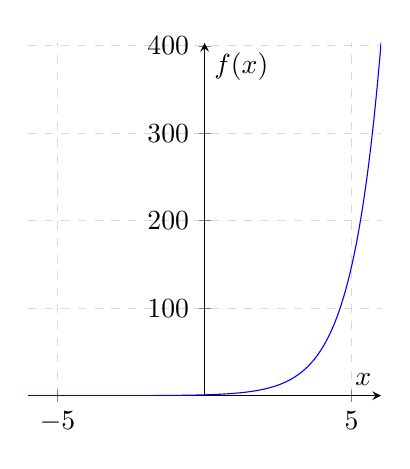
\begin{tikzpicture}
		\begin{axis}[
		samples=1000, 
		domain=-6:6,
		%	title=Niveaulinien von $F$,
		x label style={at={(axis description cs:1, 0)}, right},
		y label style={at={(axis description cs:0, 1)}, left, rotate=-90},
		xlabel=$x$,
		ylabel=$f(x)$,
		grid, 
		grid style={dashed,gray!30},
		axis y line=center,
		axis x line=center,
		xmin = -6,
		xmax = 6,
		width=0.5\textwidth,
		height=0.5\textwidth
		]
		\addplot[blue] {exp(x)};
		\end{axis}
		\end{tikzpicture}
	\end{center}
	% Here ends the furst plot
	
\end{beispiel}

We continue with defining an inequality for uniformly convex functions, which will be useful later on.

\begin{lemma}
	Let $f:\R^n\rightarrow\R$ be continuously differentiable, $x_0 \in\R^n$, the level set $\mathcal{L}(x_0)$ convex, $f$ uniformly convex on $\mathcal{L}(x_0)$ and $x \in\R$, according to Theorem 2, 3), unique global minimum of $f$. Then there exists $\mu>0$ with
	\begin{align*}
	\mu \left\lVert x-x^* \right\Vert^2 \leq f(x)-f(x^*) \qquad \forall \bigskip x \in \mathcal{L}(x_0)
	\end{align*}. 
\end{lemma}

\begin{proof}
	Using: 
	\begin{itemize}
		\item The inequality \labelcref{definition:3:strictlyconvex} from the begining of this lecture and 
		\item the fact that $x^*$ is, as a result of being a global Minimum of $f$, a stationary point of f and therefore $\nabla f(x^*)=0$,
	\end{itemize}
	we conclude the needed inequality.
\end{proof}

Finally, we analyze in which way the existence of stationary points of a function are connected to the existence of global minimum of that function.

\begin{satz}
	Let $f:\R^n\rightarrow\R$ be continuously differentiable and convex function, $x\in\R^n$ a stationary point of $f$. Then $x^*$ is a global minimum of $f$ on $\R^n$. 
\end{satz}

\begin{proof}
	First, we remind ourselves that a point $x^*\in X$ is called a stationary point of a continiously differentiable function $f:\R^n\rightarrow\R$, if $\nabla f(x^*)=0$.
	From Proposition 3.5. a) follows: 
	\begin{align*}
	f(x)-f(x^*)\leq\nabla f(x^*)^t (x^*)=0
	\end{align*}
	and thus 
	\begin{align*}
	f(x)\geq f(x^*), \forall x\in R
	\end{align*}
	It follows that $x^*$ is a global minimum of $f$.
\end{proof}
    \chapter{Allgemeines Abstiegsverfahren}

Gesucht ist ein Verfahren zur Lösung des Problems $\min f(x)$, $x \in \R^n$ mit $\abb{f}{\R^n}{\R}$.

Idee: Man ermittelt zu einem Punkt $x \in \R^n$ eine Richtung $d \in \R^n$, in die $f(x)$ absteigt und verkleinert in dieser $f(x)$ hinreichend.

\begin{definition}[Abstiegsrichtung] \label{definition: 6.1}
	Sei $\abb{f}{\R^n}{\R}$ eine stetig differenzierbare Funktion, $x \in \R^n$. Ein Vektor $d \in \R^n$ heißt Abstiegsrichtung von $f$ in $x$, wenn es ein $\quer{t} > 0$ gibt mit $f(x + td) < f(x)$ für alle $t \in (0,\quer{t})$.
\end{definition}

\begin{lemma} \label{lemma: 6.2}
	Sei $\abb{f}{\R^n}{\R}$ stetig differenzierbar, $x \in \R^n$, $d \in \R^n$ mit $\nabla \trans{f(x)} d < 0$. \\
	$\follows d$ ist eine Abstiegsrichtung
\end{lemma}
\begin{proof}
	Da $f$ ist stetig differenzierbar ist, folgt für die Richtungsableitung $f'(x;d)$
	\begin{equation*}
		f'(x;d) = \lim_{t \to 0} \frac{f(x + td)-f(x)}{t} = \nabla \trans{f(x) d} < 0
	\end{equation*}
	Somit ist $\frac{f(x+td)-f(x)}{t} <0$ für hinreichend kleine $t$.
\end{proof}

\begin{bemerkung}
	\cref{lemma: 6.2} ist ein hinreichendes aber kein notwendiges Kriterium für eine Abstiegsrichtung. Ist beispielsweise $x \in \R^n$ ein striktes lokales Maximum eine beliebiegen Funktion $f$, so ist nach \cref{definition: 6.1} jedes $0 \neq d \in \R^n$ eine Abstiegsrichtung, jedoch ist die Bedingung von \labelcref{lemma: 6.2} nicht erfüllt, da $\nabla f(x) = 0$.
\end{bemerkung}

\begin{beispiel}
	Sei $\abb{f}{\R^n}{\R}$ stetig differenzierbar, $x \in \R^n$ mit $\nabla f(x) \neq 0$. Dann ist $d = - \nabla f(x)$ nach \cref{lemma: 6.2} eine Abstiegsrichtung. Allgemeiner ist auch $d = - B * \nabla f(x)$ mit einer symmetrischen, positiv definiten Matrix $B \in \R^{n \times n}$ eine Abstiegsrichtung.
\end{beispiel}

\begin{algorithmus} \label{algorithmus: 6.5}
	\begin{enumerate}[leftmargin=*, label=Schritt \arabic*., nolistsep]
		\item Wähle $x^0 \in \R^n$ und setze $k \defeq 0$.
		\item Wenn $x^k$ einem Abbruchkriterium genügt: Stop.
		\item Bestimme $d^k$ von $f$ in $x$.
		\item Bestimme $t^k > 0$ mit $f(x^k + t^k d^k) < f(x^k)$.
		\item Setze $x^{k+1} = x^k + t^k d^k$, $k \to k+1$, gehe zu Schritt 1.
	\end{enumerate}
\end{algorithmus}

Implizit nehmen wir im Folgenden an, dass dieser Algorithmus eine unendliche Folge $\folge[k \in \N]{x^k}$ generiert.

\begin{definition}
	Sei $\abb{f}{\R^n}{\R}$ stetig differenzierbar, $x \in \R^n$, $d \in \R^n$ eine Abstiegsrichtung von $f$ in $x$.
	\begin{itemize}[leftmargin=*, nolistsep]
		\item Eine Abbildung $\abb{T}{\R^n \times \R^n}{\pows{\R_+}}$ heißt \begriff{Schrittweitenstrategie}. Diese heißt wohldefiniert, wenn für $(x,d) \in \R^n \times \R^n$ mit $\nabla\trans{f(x)} d < 0$ gilt, dass $T(x,d) \neq \emptyset$.
		\item $T$ heißt \begriff{effizient}, falls es eine von $x$ und $d$ unabhängige Konstante $\theta > 0$ gibt mit
		\begin{equation*}
			f(x+ + td) \le f(x) - \theta \left( \frac{\nabla \trans{f(x)} d}{ \norm{d}} \right) \qquad \text{für alle } t \in T(x,d)
		\end{equation*}
		Eine Schrittweite $t$ heißt effizient, wenn sie mit einer effizienten Schrittweitenstrategie erzeugt wurde.
	\end{itemize}
\end{definition}

\begin{satz} \label{satz 6.7}
	Sei $\abb{f}{\R^n}{\R}$ stetig differenzierbar und $\folge[k \in \N]{x^k}$ eine Folge, die mit \cref{algorithmus: 6.5} erzeugt wurde. Außerdem gelte:
	\begin{enumerate}[label=\arabic*., nolistsep]
		\item Es existiert eine Konstante $c > 0$ mit 
		\begin{equation}
			- \frac{\trans{\nabla f(x^k)} d^k}{\norm{\nabla f(x^k)} * \norm{d^k}} \ge c \text{für allef} k \in \N \tag{\text{Winkelbedingung}}
		\end{equation}
		\item Die Schrittweiten $t^k$ seien effizient für alle $k \in \N$.
	\end{enumerate}
	Dann ist jeder Häufungspunkt der Folge $\folge[k \in \N]{x^k}$ ein stationärer Punkt von $f$.
\end{satz}
\begin{proof}
	Da alle $t^k$ effizient sind, folgt die Existenz eines $\theta > 0$ mit
	\begin{equation*}
		f(x^{k+1}) = f(x^k + t^k d^k) \le f(x^k) - \theta \left( \frac{\trans{\nabla f(x^k)} d^k}{\norm{d^k}} \right)^2 \quad \text{für alle } k \in \N
	\end{equation*}
	Mit der Winkelbedingung folgt nun
	\begin{equation*}
		f(x^{k+1}) \le f(x^k) - \theta c^2 \norm{\nabla f(x^k)}^2
	\end{equation*}
	Sei $x^\ast$ Häufungspunkt von $\folge[k \in \N]{x^k}$. Es ist klar, das $\folge[k \in \N]{f(x^k)}$ monoton fallend ist und zumindest eine Teilfolge gegen $f(x^\ast)$ konvergiert. Damit konvergiert dann auch $f(x^k) \to f(x^\ast)$. Insbesondere gilt $f(x^{k+1}) - f(x^k) \to 0$ und $\norm{\nabla f(x^k)} \to 0$. Somit ist jeder Häufungspunkt von $\folge[k \in \N]{x^k}$ ein stationärer Punkt von $f$.
\end{proof}

\begin{beispiel}
	Sei $\abb{f}{\R^n}{\R}$ eine quadratische Funktion, d.h. $f(x) \defeq \lfrac{1}{2} \trans{x}Qx + \trans{c}x + \gamma$ mit $Q \in \R^{n \times n}$ symmetrisch und positiv definit. Seien $x \in \R^n$ und $d \in \R^n$ eine Abstiegsrichtung, die beliebig gegeben sind. Dann liefert 
	\begin{equation*}
		t_{\min} = - \frac{\nabla \trans{f(x)} d}{\trans{d} Q d}
	\end{equation*}
	den stärksten Abstieg.
\end{beispiel}
\begin{proof}
	Sei $t \in \R$. Es ist $f(x + td) = f(x) + t \nabla \trans{f(x)} d + \lfrac{1}{2} t^2 * \trans{d} Q d$. Definieren wir $\phi(t) \defeq f(x + td)$, dann ist $\phi'(t_{\min}) = 0$. Daraus folgt nun
	\begin{equation*}
		0 = \phi'(t_{\min}) = \nabla \trans{f(x)} d + t_{\min} \trans{d} Q d \quad \follows \quad t_{\min} = - \frac{\nabla \trans{f(x)} d}{\trans{d} Q d}
	\end{equation*}
	Nun kann man noch zeigen, dass $t_{\min}$ effizient ist:
	\begin{equation*}
		\begin{aligned}
		f(x + t_{\min} d) &= f(x) + t_{\min} \nabla \trans{f(x)} d + \frac{1}{2} t_{\min}^2 \trans{d} Q d \\
		&= f(x) - \frac{1}{2} t_{\min}^2 \trans{d} Q d \\
		&= f(x) - \frac{\left( \nabla \trans{f(x)} d \right)^2}{2 \trans{d} Q d}
		\end{aligned}
	\end{equation*}
	Damit gilt offensichtlich, dass ein $\theta$ exisitert mit $\frac{1}{2 \trans{d} Q d} \ge \frac{\theta}{\norm{d}^2}$
\end{proof}
    \chapter{Fortsetzung Abstiegsverfahren}

\newcommand{\level}{\mathcal{L}}

\begin{satz} \label{satz 7.1}
	Seien $x_0 \in \R^n$, $\abb{f}{\R^n}{\R}$ stetig differenzierbar, die Levelmenge $\L (x^0) \defeq \menge{x \in \R^n \colon f(x) \le f(x^0)}$ konvex und $f$ gleichmäßig konvex auf $\L(x^0)$. Sei $\folge{x^k}$ eine durch den \cref{algorithmus: 6.5} (Abstiegsverfahren) erzeugte Folge, sodass
	\begin{enumerate}
		\item Es ist $\sum_{k=0}^{\infty} \delta_k = \infty$ wobei
		\begin{equation*}
			\delta_k \defeq \left( \frac{\nabla \trans{f(x^k)} d^k}{\norm{\nabla f(x^k)} \norm{d^k}} \right)^2 \tag{Zoutendijk-Bedingung}
		\end{equation*}
		\item Die Schrittweiten $t_k > 0$ sind effizient für alle $k \in \N$. 
	\end{enumerate}
	Dann konvergiert die Folge $\folge{x^k}$ gegen das eindeutig bestimmte globale Minimum von $f$.
\end{satz}
\begin{proof}
	Sei $k \in \N$. Wegen $x^0 \in \level(x^0)$ gilt $\level(x^0) \neq \emptyset$ und mit \cref{lemma3.9} folgt, dass $\level(x^0)$ kompakt. Da jedes globale Minimum von $f$ azf dem $\R^n$ notwendig in der Levelmenge $\level(x^0)$ liegen muss, besitzt $f$ nach Theorem 5.4 genau ein globales Minimum $x^\ast$. Da $f$ gleichmäßig konvex auf $\level(x^0)$ ist, existiert ein $\mu > 0$, sodass für alle 
	\begin{equation}
		\forall x,y \in \level(x^0): f(x) - f(y) \ge \nabla \trans{f(y)}(x-y) + \mu \norm{x-y}^2 \label{eq: satz_7.1_1}
	\end{equation}
	Aus der trivialen Ungleichung
	\begin{equation*}
		0 \le \norm{\sqrt{\frac{\mu}{2}} (x^\ast - x^k) + \sqrt{\frac{1}{2\mu}} \nabla f(x^k)}^2
	\end{equation*}
	folgt nach kurzer Rechnung
	\begin{equation*}
		- \frac{1}{2\mu} \norm{\nabla f(x^k)} ^2 \le \frac{\mu}{2} \norm{x^\ast - x^k}^2 + \nabla \trans{f(x^k)} (x^\ast - x^k) \le f(x^\ast) - f(x^k) 
	\end{equation*}
	Daraus folgt nun 
	\begin{align}
		- \norm{\nabla f(x^k)}^2 \le 2 \mu (f(x^\ast) - f(x^k)) \label{eq: satz_7.1_2}
	\end{align}
	Aus der Effizienz der Schrittweiten $t_k$ existiert ein $\theta > 0$ mit 
	\begin{align}
		f(x^{k+1}) &= f(x^k + t_k d^k) \notag \\
		&\le f(x^k) - \theta \left(  \frac{\nabla f(x^k) d^k}{\norm{d^k}} \right)^2 * \frac{\norm{\nabla f(x^k)}}{\nabla f(x^k)} \notag\\
		&= f(x^k) - \theta \delta_k * \norm{\nabla f(x^k)}^2 \notag \\
		\overset{\eqref{eq: satz_7.1_2}}&{\le} f(x^k) - 2\mu \theta (f(^\ast) - f(x^k))
	\end{align}
	Also ist
	\begin{equation*}
		0 \le f(x^{k+1}) - f(x^k) \overset{\eqref{eq: satz_7.1_2}}{\le} f(x^k) - 2 \delta_k \theta (f(x^k) - f(x^\ast)) - f(x^\ast) = (1 - 2 \mu \theta \delta_k) (f(x^k) - f(x^\ast))
	\end{equation*}
	Durch $k+1$-fache Anwendung dieser Ungleichung sowie unter AUsnutzung der bekannten Ungleichung $\exp(x) \ge 1 + x$ für alle $x \in \R$. Für $x = - 2 \mu \theta \delta_k$ ergibt sich
	\begin{equation}
		\begin{aligned}
		0 &\le f(x^{k+1}) - f(x^\ast) \\
		&\le \prod_{j=0}^k (1-2 \mu \theta \delta_j) (f(x^0) - f(x^\ast)) \\
		&\le \prod_{j=0}^{k} \exp(-2\mu\theta \delta_j) (f(x^0) - f(x^\ast)) \\
		&= \exp \left( -2 \mu \theta \sum_{j=0}^k \delta_j \right) (f(x^0) - f(x^\ast))                          (6)
		\end{aligned}
	\end{equation}
	Wegen $\sum_{j=0}^k \delta_j \overset{k \to \infty}{\longrightarrow} \infty$ ergibt sich hieraus die Konvergenz von $\folge{f(x^k)}$ gegen $f(x^\ast)$. Aus Lemma 5.6 folgt $0 \le \mu \norm{x^k - x^\ast}^1 \le f(x^k) - f(x^\ast)$ für alle $k \in \N$ und damit folgt auch die Konvergenz $x^k \to x^\ast$.
\end{proof}

\begin{bemerkung}
	Die Winkelbedingung aus \cref{satz 6.7} ist hinreichend für die Zoutendijk-Bedingung, denn 
	\begin{equation*}
		\exists c > 0 \enskip \forall k \in \N \colon - \frac{\nabla f(x^k) d^k}{\norm{\nabla f(x^k)} * \norm{d^k}} \ge c \quad \follows \quad \forall k \in \N \colon \delta_k \ge c^2 \ge 0 \quad \follows \sum_{j=0}^\infty \delta_j \ge \sum_{j=0}^\infty c^2 = \infty
	\end{equation*}
\end{bemerkung}

\begin{bemerkung}
	Die beiden Konvergenzsätze \cref{satz 6.7} und \labelcref{satz 7.1} sind von fundamentaler Bedeutung zum Nachweis der globalen Konvergenz verschiedener Abstiegsverfahren.
\end{bemerkung}

\begin{folgerung}
	Seien $x_0 \in \R^n$, $\abb{f}{\R^n}{\R}$ stetig differenzierbar, die Levelmenge $\level(x^0) \defeq \menge{x \in \R^n \colon f(x) \le f(x^0)}$ konvex und $f$ gleichmäßig konvex auf $\level(x^0)$. Sei $\folge{x^k}$ eine durch den \cref{algorithmus: 6.5} (Abstiegsverfahren) erzeugte Folge, sodass
	\begin{enumerate}
		\item $\exists \delta > 0 \enskip \forall k \in \N \colon \delta_k \ge \delta$ wobei
		\begin{equation*}
		\delta_k \defeq \left( \frac{\nabla \trans{f(x^k)} d^k}{\norm{\nabla f(x^k)} \norm{d^k}} \right)^2
		\end{equation*}
		\item Die Schrittweiten $t_k > 0$ sind effizient für alle $k \in \N$. 
	\end{enumerate}
	Dann konvergiert die Folge $\folge{x^k}$ gegen das eindeutig bestimmte globale Minimum $x^\ast$ von $f$ und es existieren Konstanten $c \ge 0$ und $q \in (0,1)$ mit $\norm{x^k - x^\ast} \le cq^k$ für alle $k \in \N$ (d.h. $\folge{x^k}$ konvergiert R-linear gegen $x^\ast$).
\end{folgerung}

\begin{proof}
	\begin{equation*}
		\forall k \in \N \colon \delta_k \ge \delta \follows \forall k \in \N \colon \sum_{j=0}^k \delta_j \ge \delta (k+1) \follows \sum_{j=0}^k \delta_j \overset{k \to \infty}{\longrightarrow} \infty
	\end{equation*}
	Mit \cref{satz 7.1} folgt die Konvergenz von $\folge{x^k}$ gegen $x^\ast$. Weiterhin gilt für alle $k \in \N$ mit Lemma 5.6
	\begin{align*}
		\mu \norm{x^k - x^\ast}^2 &\le f(x^k) - f(x^\ast) \\
		&\le \exp \left( - 2 \mu \theta \sum_{j=0}^{k-1} \delta_j \right) (f(x^0) - f(x^\ast)) \\
		&\le \exp \left( -2 \mu \theta \delta * k \right) (f(x^0) - f(x^\ast)) \\ \follows \quad \norm{x^k - x^\ast} &\le \sqrt{\frac{(f(x^0) - f(x^\ast))}{\mu} * \exp(-2\mu \theta \delta k)} = \underbrace{\sqrt{\frac{(f(x^0) - f(x^\ast))}{\mu}}}_{\defqe c} * \underbrace{\exp(-\mu \theta \delta)}_{\defqe q}^k
	\end{align*}
\end{proof}
    \newcommand{\nat}{\mathbb{N}}				% natürliche Zahlen
\newcommand{\integer}{\mathbb{Z}}			% ganze Zahlen
\newcommand{\ratio}{\mathbb{Q}}
\newcommand{\real}{\mathbb{R}}				% reelle Zahlen
\newcommand{\complex}{\mathbb{C}}			% komplexe Zahlen
\newcommand{\korper}{\mathbb{K}}            % Körper IR oder IC


\chapter{Schrittweitenstrategien}

\vortragender{Lars Ortscheidt}

Das bisher kennengelernte Abstiegsverfahren hat in Bezug auf die Abstiegsrichtung $d$ und die Schrittweite $t$ große Freiheitsgrade. Da die Schrittweite $t_{\min}$ mit $f(x+t_{\min}d) = \min_{t\geq 0} f(x+td)$ im Allgemeinen nicht in endlich vielen Schritten berechnet werden kann, werden nun zwei Schrittweitenregeln vorgestellt, welche ''realisierbar`` sind, d.h. sie brauchen nur endlich viele Schritte zur Berechnung.


\section{Armijo-Regel}

\begin{definition}
	Seien $f: \real^n \to \real$ stetig differenzierbar und $\sigma, \beta \in (0,1)$ fest für das ganze Abstiegsverfahren. Zu $x, d \in \real^n$ mit $\nabla f(x)^{\top} d<0$ bestimme $t \defeq \max_{\ell \in \nat_0} \beta^\ell$, so dass gilt 
	\begin{align}
		f(x+td) \leq f(x) + \sigma t \nabla f(x)^{\top} d.  \label{armijo}
	\end{align}	 
	Dieses Verfahren heißt \begriff{Armijo-Regel}. \\
	Setzt man $\phi(t) := f(x+td)$ lautet \labelcref{armijo} 
	\begin{align*}
		\phi(t) \leq \phi (0) + \sigma t \phi' (0),
	\end{align*}
	die sogenannte Armijo-Goldstein-Bedingung.
\end{definition}

\begin{bemerkung}
	\begin{itemize}	
		\item Zur Bestimmung von $t$ wird \labelcref{armijo} also für $t= \beta^\ell$, $\ell=0,1,2,...$ überprüft und bei der ersten Gültigkeit abgebrochen.
		\item $T(x,d)$ besitzt bei der Armijo-Regel höchstens ein Element.
	\end{itemize}
\end{bemerkung}
\begin{satz}
	Seien $f: \real^n \to \real$ stetig differenzierbar mit $\sigma , \beta \in (0,1)$, fest. Dann existiert für alle $x,d \in \real^n$ mit $\nabla f(x)^{\top} d < 0$ ein endliches $\ell \in \nat$ mit
	\begin{align*}
		f(x+ \beta^\ell d) \leq f(x)+ \sigma \beta^\ell \nabla f(x)^{\top} d, 
	\end{align*}
	d.h. die Armijo-Regel ist wohldefinitionniert.
\end{satz}

\begin{proof}
	Angenommen für alle $\ell \in \nat$ gilt
	\begin{align*}
		f(x+ \beta^\ell d) > f(x)+ \sigma \beta^\ell \nabla f(x)^{\top} d
	\end{align*}
	und somit auch
	\begin{align*}
		\frac {f(x+ \beta^\ell d) - f(x)}{\beta^\ell} > \sigma \nabla f(x)^{\top} d.
	\end{align*}
	Dann folgt mit $\ell \to \infty$ wegen der Differenzierbarkeit von $f$
	\begin{align*}
		\nabla f(x)^{\top} d > \sigma \nabla f(x)^{\top} d
	\end{align*}
	und weil $\sigma \in (0,1)$ ergibt sich
	\begin{align*}
		\nabla f(x)^{\top} d \geq 0,
	\end{align*}
	was im Widerspruch zur Voraussetzung des Satzes steht.
\end{proof}


\section{Wolfe-Powell-Schrittweitenstrategie}

\begin{definition}
	Seien $f: \real^n \to \real$ stetig differenzierbar und $\sigma \in (0, \frac{1}{2}), \, \rho \in [\sigma, 1)$ fest vorgegeben. Für $x,d \in \real^n$ mit $\nabla f(x)^{\top} d <0$ bestimme man ein $t >0$ mit 
	\begin{align}
		f(x+td) \leq f(x) + \sigma t \nabla f(x)^{\top} d \label{w_p_1}
	\end{align}
	und
	\begin{align}
		\nabla f(x+td)^{\top} d \geq \rho \nabla f(x)^{\top} d. \label{w_p_2}
	\end{align}
	\labelcref{w_p_1} und \labelcref{w_p_2} heißen dann die \begriff{Wolfe-Powell-Bedingungen}. \\ Setzt man $\phi(t) := f(x+td)$, so lauten \labelcref{w_p_1} und \labelcref{w_p_2}
	\begin{align*}
		\phi (t) \leq \phi (0)+\sigma t \phi' (0)
	\end{align*}
	und
	\begin{align*}
		\phi'(t) \geq \rho \phi' (0).
	\end{align*}
\end{definition}

\begin{satz}
	Seien $f:\real^n \to \real$ stetig differenzierbar und $\sigma \in (0, \frac{1}{2})$, $\rho \in [\sigma, 1)$, $x^0 \in \real^n$ fest. Zu $x \in \mathcal{L}(x^0) := \{ z \in \real^n | f(z) \leq f(x^0) \}$ und $d \in \real^n$ mit $\nabla f(x)^{\top} d <0$ sei 
	\begin{align*}
		T_{WP} (x,d) := \{ t>0 | \text{\labelcref{w_p_1} und \labelcref{w_p_2} gelten} \}
	\end{align*}
	die Menge der Wolfe-Powell-Schrittweiten in $x$ in Richtung $d$. Dann gelten:
	\begin{enumerate}[label=(\alph*)]
	\item Ist f nach unten beschränkt, so ist $T_{WP}(x,d) \neq \emptyset$, d.h. die Wolfe-Powell-Strategie ist wohldefinitionniert.
	\item Ist außerdem der Gradient $\nabla f$ auf der Levelmenge $\mathcal{L}(x^0)$ Lipschitz-stetig, so existiert eine Konstante $\theta >0$ (unabhängig von x und d) mit
	\begin{align*}
		f(x+td) \leq f(x) - \theta \left( \frac{\nabla f(x)^{\top} d}{\| d \|}     \right)^2
	\end{align*}	 
	für alle $t \in T_{WP}(x,d)$, d.h. die Wolfe-Powell-Schrittweitenstrategie ist effizient.
	\end{enumerate}
\end{satz}

\begin{proof}
	Zu (a): Setze 
	\begin{align*}
		\phi(t) &:= f(x+td), \\
		\psi (t) &:= f(x+td)-f(x)- \sigma t \nabla f(x)^{\top} d= \phi(t) - \phi(0) - \sigma t \phi'(0) 
	\end{align*}
	und somit
	\begin{align*}
		\phi'(t) = \nabla f(x+td)^{\top} d, \\
		\psi'(t) = \phi'(t) - \sigma \phi'(0).
	\end{align*}
	So lauten \labelcref{w_p_1} und \labelcref{w_p_2}
	\begin{align}
		\psi (t) &\leq 0 \label{w_p_3} \\
		\phi'(t) &\geq \rho \phi'(0) \label{w_p_4}.
	\end{align}
	Offenbar gilt $\psi(0)=0, \lim_{t \to \infty} \psi(t) = \infty$ (da $f$ beschränkt), $\psi'(0) <0$, damit $\psi'(t) <0$ für $t \in [0, t_0), t_0 >0$. Daher existiert $t^\ast>0$ minimal mit $\psi(t^\ast)=0, \psi(t)<0$ für $t \in (0,t^\ast)$, somit erfüllt $t^\ast$ \labelcref{w_p_3}. Da $\psi'(t^\ast) \geq 0$ folgt $\phi'(t^\ast) \geq \sigma \phi'(0)$, womit wegen $\rho \geq \sigma >0$ und $\phi'(0)<0$ \labelcref{w_p_4} für $t^\ast$ folgt, also $t^\ast \in T_{WP}(x,d).$ 
	\\ 
	Zu (b): Sei $t \in T_{WP}(x,d)$ gegeben. Dann ist $f(x+td) \leq f(x)$ und somit insbesondere $x+td \in \mathcal{L}(x^0)$. Aus der Wolfe-Powell-Regel folgt zunächst
	\begin{align*}
		\rho \nabla f(x)^{\top} d - \nabla f(x)^{\top} d &\leq \nabla f(x+td)^{\top} d - \nabla f(x)^{\top} d \\
		\Longleftrightarrow \qquad (\rho -1) \nabla f(x)^{\top}d &\leq ( \nabla f(x+td)- \nabla f(x) )^{\top} d.
	\end{align*}
	Mit der Cauchy-Schwarzschen Ungleichung und vorausgesetzten Lipschitz-Stetigkeit von $\nabla f(x)$ auf $\mathcal{L}(x^0)$ folgt mit einer geeigneten Konstanten $\ell > 0$:
	\begin{align*}
		(\rho -1) \nabla f(x)^{\top}d \leq \| \nabla f(x+td)- \nabla f(x) \| \; \|d\| \leq Lt \|d\|^2
	\end{align*}
	Hieraus folgt
	\begin{align*}
		t \geq \frac{(\rho -1) \nabla f(x)^{\top} d}{\ell \|d\| ^2}
	\end{align*}
	und daher 
	\begin{align*}
		f(x+td) &\mathop{\leq}^{\labelcref{w_p_1}} f(x) + \sigma  t \nabla f(x)^{\top} d \\
		&\leq f(x)+ \sigma \frac{(\rho -1) \nabla f(x)^{\top} d}{\ell \|d\| ^2} \nabla f(x)^{\top} d \\
		&\leq f(x) - \theta \left(\frac{\nabla f(x)^{\top} d}{\|d\|}\right)^2
	\end{align*}
	mit 
	\begin{align*}
		\theta := \frac{(1-\rho) \sigma}{\ell}
	\end{align*}
	Damit ist die Behauptung bewiesen.
\end{proof}

Abschließend zwei hinreichende Bedingungen dafür, dass der Gradient $\nabla f$ auf der Levelmenge $\mathcal{L}(x^0)$ Lipschitz-stetig ist.
\begin{lemma}
	Seien $f: \real^n \to \real$ zweimal stetig differenzierbar und $x^0 \in \real^n$. Ist eine der folgenden Bedingungen erfüllt:
	\begin{enumerate}
	\item[(a)] $\| \nabla^2 f(x) \|$ ist beschränkt auf einer konvexen Obermenge $X$ der Levelmenge $\mathcal{L}(x^0)$,
	\item[(b)] die Levelmenge $\mathcal{L}(x^0)$ ist kompakt,
	\end{enumerate}
	so ist der Gradient $\nabla f$ Lipschitz-stetig auf $\mathcal{L}(x^0)$. 
\end{lemma}

\begin{proof}
	Sei Bedingung (b) erfüllt. Definiere 
	\begin{align*}
		[\mathcal{L}(x^0)]:= \{ ax+(1-a)y \mid a \in [0,1], x,y \in \mathcal{L}(x^0) \},
	\end{align*} offenbar ist diese Menge eine konvexe Obermenge von $\mathcal{L}(x^0)$. Betrachte die Funktion  
	\begin{align*}
	f \colon \left\lbrace%	
	\begin{array}{ccl}%
		[0,1] \times \mathcal{L}(x^0) \times \mathcal{L}(x^0) & \to & [\mathcal{L}(x^0)] \\%
		(a,x,y) & \mapsto & ax+(1-a)y%
	\end{array}%
\right.
	\end{align*}
	Offenbar ist f stetig und surjektiv mit kompaktem Definitionsbereich. Da das Bild von kompakten Mengen unter stetigen Funktionen wieder kompakt ist, folgt $[\mathcal{L}(x^0)]$ kompakt, d.h. es es existiert eine konvexe und kompakte Obermenge $X \subseteq \real^n$ mit $\mathcal{L}(x^0) \subseteq X$.
	Aus Stetigkeitsgründen existiert dann eine Konstante $L$ mit 
	\begin{align}
		\| \nabla^2 f(x)\| \leq L \qquad \text{ für alle } x \in X, \label{wa}
	\end{align}
	d.h. die Bedingung (a) ist erfüllt. \\
	Sei nun die Bedingung (a) erfüllt. Dann existiert eine Zahl $L>0$ mit \labelcref{wa} . Es gilt
	\begin{align*}
		 \int_{0}^{1} \nabla^2 f(y+ \tau(x-y))(x-y) \, d \tau = \left[\nabla f(y+ \tau(x-y))\right]_{\tau =0}^1 = \nabla f(x) - \nabla f(y)
	\end{align*}
	für alle $x,y\in X$. Wegen $y+\tau (x-y) \in X$ ist daher
	\begin{align*}
		\| \nabla f(x) - \nabla f(y) \| &\leq \int_{0}^{1} \| \nabla^2 f(y+ \tau(x-y)) \|  \, d \tau \, \|x-y\| \\
		&\leq \int_0^1 L \, d\tau \, \| x-y \| \\
		&= L \| x-y \|
	\end{align*}
	für alle $x,y \in X$, was zu zeigen war. 
\end{proof}

\undef\nat
\undef\integer
\undef\ratio
\undef\real
\undef\complex
\undef\korper
    \chapter{Schrittweitenalgorithmen}
\vortragender{Michael Kunert}

\begin{erinnerung}
	Sei $\abb{f}{\R^n}{\R}$ stetig differenzierbar und $\sigma \in (0,\frac{1}{2})$ sowie $\rho \in [0,1)$ gegeben. Zu $x,d \in \R^n$ mit $\nabla \trans{f(x)} d < 0$ bestimme man ein $t > 0$ mit 
	\begin{align}
		f(x+td) &\le f(x) + \sigma t \nabla \trans{f(x)} d \label{eq: armijo2} \\
		\nabla \trans{f(x+td)} d &\ge \rho \nabla \trans{f(x)} d \label{eq: wp}
	\end{align}
	Zur Vereinfachung im Algorithmus setzen wir im Folgenden stets
	\begin{align*}
			\phi(t) &\defeq f(x+td) \\
			\psi(t) &\defeq \phi(t) - \phi(0) - \sigma t \phi'(0)
	\end{align*}
\end{erinnerung}

\begin{bemerkung}
	Die Wolfe-Powellbedingungen \labelcref{eq: armijo2} und \labelcref{eq: wp} sind damit 
	\begin{align*}
		\psi(t) \le 0 \quad \und \quad \phi'(t) \ge \rho \phi'(0) 
	\end{align*}
\end{bemerkung}
\begin{proof}
	Zum einen ist
	\begin{alignat*}{2}
		&&\psi(t) &= \phi(t) - \phi(0) - \sigma t \phi'(0) \le 0 \\
		\equivalent &&f(x + td) - f(x) - \sigma t \trans{\nabla f(x)} d &\le 0 \\
		\equivalent &&f(x + td) &\le f(x) + \sigma t \nabla \trans{f(x)} d
	\end{alignat*}
	und außerdem
	\begin{align*}
		\phi'(t) \ge \rho \phi'(0) \equivalent \nabla \trans{f(x+td)} d \ge \rho \nabla \trans{f(x)} d
	\end{align*}
\end{proof}

\begin{lemma}
	Seien $\sigma < \rho$ und $\phi'(0) < 0$. Ist $[a,b]$ mit $0 \le a \le b$ ein Intervall mit den Eigenschaften $\psi(a) \le 0$, $\psi(b) \ge 0$ und $\psi'(a) < 0$, so enthält das Intervall $[a,b]$ einen Punkt $\quer{t}$ mit $\psi(\quer{t}) < 0$ und $\psi'(\quer{t}) = 0$. $\quer{t}$ ist ein innerer Punkt eines Intervalls $I$, sodass für alle $t \in I$ gilt:
	\begin{align}
		\psi(t) \le 0 \quad \und \quad \phi'(t) \ge \rho \phi'(0) \label{eq: 9_lemma}
	\end{align}
\end{lemma}
\begin{proof}
	Sei $\quer{t}$ ein gloables Minimum von $\psi$ auf $[a,b]$ (Satz von Weierstraß). Wegen \labelcref{eq: 9_lemma} ist $\quer{t}$ ein innerer Punkt von $[a,b]$. Außerdem ist $\psi(\quer{t})$ muss gelten. 
	Wegen $\sigma < \rho$ folgt die Existenz von $I$, sodass für alle $t \in I$ gilt
	\begin{align*}
		\left.\begin{array}{rcl}
		\psi(t) &\le & 0 \quad \und \quad \psi'(t) \ge (\rho - \sigma) \phi'(0) \\
		\psi'(t) &= & \phi'(t) - \sigma \phi'(0)
		\end{array}
		\right\} \follows \psi(t) \le 0 \quad \und \quad \phi'(t) \ge \rho \phi'(0) \enskip \forall \ t \in I
	\end{align*}
\end{proof}

\begin{algorithmus} \label{alg}
	Gegeben seien $x \in \R^n$ und $d \in \R^n$ mit $\nabla \trans{f(x)} d < 0$. 
	\begin{enumerate}[label=Phase~\Alph*., leftmargin=4.5em, nolistsep]
		\item ~
		\begin{enumerate}[label=\Alph{enumi}.\arabic*, start=0]
			\item Wähle $t_0 > 0$, $\gamma > 1$ und setze $i \defeq 0$.
			\item Ist $\psi(t_i) \ge 0$, so setze $a \defeq 0$ und $b \defeq t$ und gehe zu (B.0). \\
			Ist $\psi(t_i) < 0$, $\psi'(t_i) \ge \rho \phi'(0)$, so setze $t \defeq t_i$ und breche ab. \texttt{STOP 1}. \\
			Ist $\psi(t_i) < 0$, $\psi'(t_i) < \rho \phi'(0)$, so setze $t_{i+1} \defeq \gamma t$, $i = i+1$ und gehe zu (A.1)
		\end{enumerate}
		\item ~
		\begin{enumerate}[label=\Alph{enumi}.\arabic*, start=0, nolistsep]
			\item Wähle $\tau_1, \tau_2 \in (0,\frac{1}{2}]$, setze $j \defeq 0$ und setze $a_0 \defeq a$ sowie $b_0 \defeq b$.
			\item Wähle $t_j \in [a_j + \tau_1 (b_j - a_j), b_j + \tau_2 (b_j - a_j)]$.
			\item Ist $\psi(t_j) \ge 0$, so setze $a_{j+1} = a_j$, $b_{j+1} = t_j$, $j=j+1$ und gehe zu (B.1). \\
			Ist $\psi(t_j) < 0$, $\psi'(t_i) \ge \rho \phi'(0)$, so setze $t \defeq t_j$ und breche ab. \texttt{STOP 2}. \\
			Ist $\psi(t_i) < 0$, $\psi'(t_i) < \rho \phi'(0)$, so setze $a_{j+1} \defeq t_j$, $b_{j+1} \defeq b_j$, $j = j+1$ und gehe zu (B.1).
		\end{enumerate}
	\end{enumerate}
	\counterwithout{enumii}{enumi}
\end{algorithmus}

Wenn $f$ nach unten beschränkt ist und eine Schranke $\uline{f}$ bekannt ist, dann gilt
\begin{align*}
	\psi(t) \le 0 \equivalent \sigma t \phi'(0) \le \phi(t) - \phi(0) \follows t \le \frac{\uline{f} - \phi(0)}{\sigma \phi'(0)}
\end{align*}
also ist $t_0 \in (0,t)$.

\begin{satz}
	Sei $\abb{f}{\Rn}{\R}$ stetig differenzierbar und nach unten beschränkt. Des Weiteren seien $\sigma \in (0,\frac{1}{2})$ und $\rho \in (\sigma , 1)$. Dann bricht \cref{alg} nach endlich vielen Schritten ab.
\end{satz}
\begin{proof}
	\begin{enumerate}[label=Phase~\Alph*:, nolistsep, leftmargin=*]
		\item Bricht \cref{alg} bei \texttt{STOP 1} ab, dann sind die Wolfe-Powell-Bedingungen erfüllt. Bei der Übergabe nach (B.0) hat $[a,b]$ offenbar die Eigenschaften \labelcref{eq: 9_lemma} und $\phi'(a) < \sigma \phi'(0)$. Angenommen Phase A würde nicht abbrechen. Dann ist für $t_i = \gamma^i * t_0$ aufgrund der Fallvoraussetzung $\psi(t_i) < 0$, also $\phi(t_i) < \phi(0) + \sigma t_i \phi'(0)$. Das ist wegen $\gamma > 1$, $\phi'(0) < 0$ und der Beschränkung von $f$ nicht möglich.
		\item Wenn Phase B bei \texttt{STOP 2} abbricht, sind die Wolfe-Powell-Bedingungen erfüllt. Zeige nun, dass für alle Intervalle $[a_j, b_j]$ die Gleichung \eqref{eq: 9_lemma} erfüllt und $\phi'(a_j) < \rho \phi'(0)$ mittels Induktion. Für $j = 0$ ist die Aussage erfüllt. Habe nun $[a_j, b_j]$ die geforderten Eigenschaften. Falls $\phi(t_j) \ge 0$ gilt $\psi(a_{j+1}) \le 0$, $\psi(b_{j+1}) \ge 0$ und $\psi'(a_{j+1}) < 0$. Falls $\psi(t_j) < 0$, dann ist $\psi(a_{j+1}) \le 0$, $\psi(b_{j+1}) \ge 0$ und $\psi'(a_{j+1}) = \psi'(t_j) < \rho \phi'(0) < 0$. In beiden Fällen sind die Eigenschaften also erfüllt. 
		
		Es bleibt zu zeigen, dass auch auch Phase B abbricht. Die Intervalllängen $\abs{b_j - a_j}$ ziehen sich auf einen Punkt $t^\ast$ zusammen. Nach Lemma 9.2 gibt es jedem $[a_j,b_j]$ ein $t_j \in (a_j,b_j)$ mit $\psi(t_j) < 0$ und $\psi'(t_j) = 0$. Wegen $t_j \to t$ für $j \to \infty$ folgt $\psi'(t^\ast) = 0$, also $\phi(t^\ast) = \sigma \phi'(0)$. Das steht jedoch im Widerspruch zu $\phi'(a_j) < \rho \phi'(0)$ und daraus resultierend $\phi'(t^\ast) \le \rho \phi'(0)$.  
	\end{enumerate}
\end{proof}
    \chapter{Gradienten- und Gradientenähnliche Verfahren}

\vortragender{Duc Anh Nguyen}

\textbf{Motivation:} Die Richtung des steilsten Abstiegs von $\abb{f}{\Rn}{\R}$ (differenzierbar) im Punkt $x$ ist ein Vektor $d$, der folgende Optimierungsaufgabe löst:
\begin{equation*}
	\min \nabla \trans{f(x)} d \text{ unter der Nebenbedingung } \norm{d} = 1
\end{equation*}
\begin{equation*}
	\scal{\nabla f(x)}{d'} \le \norm{\nabla f(x)} * \norm{d'} = \scal{\nabla f(x)}{\frac{\nabla f(x)}{\norm{f(x)}}} \follows d = - \frac{\nabla f(x)}{\norm{\nabla f(x)}}
\end{equation*}

\begin{algorithmus} \label{algorithmus 8.1}
	\begin{enumerate}[label = Schritt \arabic*:, start=0, leftmargin = 5em, nolistsep]
		\item $x^0 \in \Rn$, $\sigma, \beta \in (0,1)$, $\epsilon \ge 0$, $k \defeq 0$.
		\item Wenn $\norm{\nabla f(x^k)} \le \epsilon$: \texttt{STOP}
		\item Setze $d^k \defeq - \nabla f(x^k)$.
		\item Bestimme $t_k \defeq \max_{\ell \in \N_0} \beta^\ell$ mit $f(x^k + t_k d^k) \le f(x^k) + \sigma t_k \nabla \trans{f(x^k)} d^k$
		\item Setze $x^{k+1} \defeq x^k + t_k d^k$, $k \leftarrow k + 1$, gehe zu Schritt 1.
	\end{enumerate}
\end{algorithmus}

\begin{lemma} \label{lemma 8.2}
	Seien $\abb{f}{\R^n}{\R}$ stetig differenzierbar und $x,d \in \Rn$, $\folge[k \in \N]{x^k}, \folge[k \in \N]{d^k} \subseteq \Rn$ mit $x_k \to x$ und $d^k \to d$, sowie $\folge[k \in \N]{t_k} \subseteq \R_{++}$ mit $t_k \to 0$. Dann ist 
	\begin{equation*}
		\lim_{k \to \infty} \frac{f(x^k + t_k d_k) - f(x^k)}{t_k} = \nabla \trans{f(x)} d
	\end{equation*}
\end{lemma}
\begin{proof}
	$\xi^k \in [x^k , x^k + t_k d^k]$ mit $f(x^k + t_k d^k) - f(x^k) = t_k \nabla \trans{f(\xi^k)} d^k$ (Mittelwertsatz). Wegen $t_k \to 0$ und $d^k \to d$ gilt $x^k + t_k d^k \to x$ und $\xi^k \to x$. Aufgrund der stetigen Differenzierbarkeit ist auch $\nabla \trans{f(\xi^k)} d \to \nabla \trans{f(x)} d$. Daraus folgt nun 
	\begin{equation*}
		\lim_{k \to \infty} \frac{f(x^k + t_k d^k) - f(x^k)}{t_k} = \lim_{k \to \infty} \nabla \trans{f(\xi^k)} d^k = \nabla \trans{f(x)} d
	\end{equation*}
\end{proof}

Für den nachfolgenden Satz setze $\epsilon = 0$, damit die erzeugte Folge $\folge[k \in \N]{x^k}$ nicht nach endlich vielen Schritten abgebrochen wird.

\begin{satz}
	Sei $\abb{f}{\Rn}{\R}$ stetig differenzierbar und $\folge[k \in \N]{x^k}$ eine von \cref{algorithmus 8.1} erzeugte Folge. Dann ist jeder Häufungspunkt von $\folge[k \in \N]{x^k}$ ein stationärer Punkt ($\nabla f(x^\ast) = 0$).
\end{satz}
\begin{proof}
	Sei $x^\ast \in \Rn$ ein Häufungspunkt von $\folge{x_k}$. Sei $\folge[K]{x_k}$ eine gegen $x^\ast$ konvergente Teilfolge von $\folge[k \in \N]{x^k}$. Dadurch konvergiert $\folge[K]{f(x^k)}$ gegen $f(x^\ast)$. Angenommen $\nabla f(x^\ast) \neq 0$. Dann ist
	\begin{equation*}
		f(x^{k+1}) = f(x^k + t_k d^k) \le f(x^k) + \sigma t_k \underbrace{\nabla \trans{f(x^k)} d^k}_{\le 0} \le f(x^k)
	\end{equation*}
	Somit ist die Folge $\folge[k \in \N]{f(x^k)}$ monoton fallend und $f(x^k) \to f(x^\ast)$. Die Folge $\folge[K]{d^k}$ konvergiert gegen $d = - \nabla f(x^\ast) \neq 0$. Weiter gilt $f(x^k) - f(x^{k+1}) \overset{k \to \infty}{\longrightarrow} 0$. Somit gilt resultierend aus Schritt 2 und Schritt 3 von \cref{algorithmus 8.1} 
	\begin{equation*}
		t_k \nabla \trans{f(x^k)} d^k = t_k \frac{f(x^k + t_k d^k) - f(x^k)}{t_k} \overset{K \ni k \to \infty}{\longrightarrow} 0
	\end{equation*}
	Somit ist $\folge[K]{t_k} \to 0$. Setze für Schritt 3 eine Folge $\folge{\ell_k}$ mit $t_k = \beta^{\ell_k}$, sodass gilt
	\begin{align*}
		&f(x^k + \beta^{\ell_k - 1} d^k) > f(x^k) + \sigma \beta^{\ell_k} \nabla \trans{f(x^k)} d^k \\
		\follows &\frac{f(x^k + \beta^{\ell_k -1} d^k) - f(x^k)}{\beta^{\ell_k - 1}} > \sigma \nabla \trans{f(x^k)} d^k \\
		\overset{\labelcref{lemma 8.2}, k \to \infty}{\follows} &- \norm{f(x^\ast)} \ge - \sigma \norm{\nabla f(x^\ast)}^2
	\end{align*}
	Dies ist nun ein Widerspruch, d.h. die Annahme war falsch und es gilt $\nabla f(x^\ast) = 0$.
\end{proof}

\begin{algorithmus} \label{algorithmus 8.5}
	Für das gradientenähnliche Verfahren wandeln wir Schritt 2 in \cref{algorithmus 8.1} ab und wählen $d^k \in \R$ mit $\nabla \trans{f(x^k)} d^k < 0$.
\end{algorithmus}

\begin{satz}
	Sei $\abb{f}{\Rn}{\R}$ stetig differenzierbar, $\folge{x_k}$ und $\folge{d^k}$ von \cref{algorithmus 8.5} erzeugte Folgen mit der Eigenschaft, dass $\folge{d^k}$ gradientenähnlich bezüglich $f$ und $\folge{x^k}$ ist, so ist jeder Häufungspunkt der Folge $\folge{x^k}$ ein stationärer Punkt von $f$.
	
	\textbf{gradientenähnlich}: es existieren Konstanten $c > 0$ und $\epsilon > 0$, sodass für alle $k \in \N$ gilt $\norm{d^k} \le c$ und $\nabla \trans{f(x^k)} d \le - \epsilon$ für alle $k \in \N$ hinreichend groß.
\end{satz}

\begin{beispiel}
	\begin{enumerate}[label=(\alph*), leftmargin=*, nolistsep]
		\item $d^k = - \nabla f(x^k)$.
		\item Sei $H$ positiv definit und symmetrisch. Setze $d^k = -H^{-1} \nabla f(x^k)$, $\nabla \trans{f(x^k)} d^k = - \nabla \trans{f(x^k)} H^{-1} \nabla f(x^k) < 0$.
	\end{enumerate}
\end{beispiel}
    
    
\end{document}
